\documentclass[aspectratio=169,11pt]{beamer}
% ==========================================================================
%  KSA lecture-slide theme  =  stock beamer "Boadilla"  +  KSA colour theme
%  brand colours sampled from the official KSA symbol mark:
%    Deep Prussian Blue  #2E3192   (지성 - intellect)
%    Golden Gray         #D6CBB1   (감성 - sensibility)
%  Engine: XeLaTeX.  Usage:
%    \documentclass[aspectratio=169,11pt]{beamer}
%    % ==========================================================================
%  KSA lecture-slide theme  =  stock beamer "Boadilla"  +  KSA colour theme
%  brand colours sampled from the official KSA symbol mark:
%    Deep Prussian Blue  #2E3192   (지성 - intellect)
%    Golden Gray         #D6CBB1   (감성 - sensibility)
%  Engine: XeLaTeX.  Usage:
%    \documentclass[aspectratio=169,11pt]{beamer}
%    % ==========================================================================
%  KSA lecture-slide theme  =  stock beamer "Boadilla"  +  KSA colour theme
%  brand colours sampled from the official KSA symbol mark:
%    Deep Prussian Blue  #2E3192   (지성 - intellect)
%    Golden Gray         #D6CBB1   (감성 - sensibility)
%  Engine: XeLaTeX.  Usage:
%    \documentclass[aspectratio=169,11pt]{beamer}
%    \input{../theme/ksa-theme.tex}
% ==========================================================================

\usepackage{fontspec}
\usepackage{amsmath,amssymb}
\usepackage{graphicx}
\graphicspath{{figs/}{../figs/}}
\usepackage{booktabs}
\usepackage{listings}

% ---- fonts (no ctex/xeCJK on this box -> fontspec drives CJK directly) -----
\defaultfontfeatures{Ligatures=TeX}
\setmainfont{Noto Sans CJK KR}
\setsansfont{Noto Sans CJK KR}
\setmonofont{Noto Sans Mono CJK KR}[Scale=0.92]

% ---- base theme: stock Boadilla ------------------------------------------
\usetheme{Boadilla}
\usefonttheme{professionalfonts}
\setbeamertemplate{navigation symbols}{}

% ---- KSA colour theme (recolour the stock theme) --------------------------
\definecolor{ksablue}{HTML}{2E3192}
\definecolor{ksabluedk}{HTML}{20226A}
\definecolor{ksagold}{HTML}{D6CBB1}
\definecolor{ksagolddk}{HTML}{A9976B}
\definecolor{ksared}{HTML}{C0392B}
\definecolor{ksagray}{HTML}{5B5B5B}

\setbeamercolor{structure}{fg=ksablue}
\setbeamercolor{alerted text}{fg=ksared}

\setbeamercolor{palette primary}{fg=white,           bg=ksablue}
\setbeamercolor{palette secondary}{fg=white,         bg=ksablue!85!black}
\setbeamercolor{palette tertiary}{fg=white,          bg=ksabluedk}
\setbeamercolor{titlelike}{fg=ksablue}
\setbeamercolor{frametitle}{fg=ksablue,bg=}
\setbeamercolor{title}{fg=ksablue}
\setbeamercolor{author}{fg=ksagray}
\setbeamercolor{institute}{fg=ksagray}
\setbeamercolor{block title}{fg=white,bg=ksablue}
\setbeamercolor{block body}{fg=black!85,bg=ksablue!6}
\setbeamercolor{item}{fg=ksablue}
\setbeamercolor{section in toc}{fg=black!85}

\setbeamerfont{frametitle}{series=\bfseries}
\setbeamerfont{title}{series=\bfseries}

% ---- footline:  KSA mark | "Made by ..." | n / N   (matches reference) ----
\newcommand{\ksacredit}{Made by Sumin Han \,\textperiodcentered\, suminhan@ksa.hs.kr}
\setbeamertemplate{footline}{%
  \hbox{%
    \begin{beamercolorbox}[wd=.18\paperwidth,ht=2.6ex,dp=1.5ex,leftskip=1.1em]{}%
      \raisebox{-0.35ex}{
\includegraphics[height=2.0ex]{ksa-logo.png}}%
    \end{beamercolorbox}%
    \begin{beamercolorbox}[wd=.64\paperwidth,ht=2.6ex,dp=1.5ex,center]{}%
      {\scriptsize\color{ksagray}\ksacredit}%
    \end{beamercolorbox}%
    \begin{beamercolorbox}[wd=.18\paperwidth,ht=2.6ex,dp=1.5ex,rightskip=1.1em]{}%
      \hfill{\scriptsize\color{ksablue}\insertframenumber\,/\,\inserttotalframenumber}%
    \end{beamercolorbox}%
  }%
  \vskip2pt
}

% ---- section divider: stock \sectionpage, KSA-coloured -------------------
\setbeamertemplate{section page}{%
  \begingroup\centering
    {\color{ksagolddk}\rule{0.16\paperwidth}{1pt}}\par\vskip1.0em
    {\usebeamerfont{title}\color{ksablue}\insertsectionhead\par}\vskip1.0em
    {\color{ksagolddk}\rule{0.16\paperwidth}{1pt}}\par
  \endgroup
}
\AtBeginSection[]{\begin{frame}[plain,noframenumbering]\vfill\sectionpage\vfill\end{frame}}

% ---- code listings ------------------------------------------------------------
\lstdefinestyle{ksa}{%
  basicstyle=\ttfamily\scriptsize,
  keywordstyle=\color{ksablue}\bfseries,
  commentstyle=\color{ksagray}\itshape,
  stringstyle=\color{ksagolddk},
  numberstyle=\tiny\color{ksagray},
  backgroundcolor=\color{ksablue!6},
  frame=leftline, framerule=1.4pt, rulecolor=\color{ksablue},
  xleftmargin=1em, aboveskip=0.8em, belowskip=0.4em,
  showstringspaces=false, breaklines=true, language=Python,
}
\lstset{style=ksa}

% ---- handy macros -----------------------------------------------------------
\newcommand{\kb}[1]{\textbf{\color{ksablue}#1}}   % blue keyword
\newcommand{\kq}[1]{\textbf{\color{ksared}#1}}    % red key-question

% ==========================================================================

\usepackage{fontspec}
\usepackage{amsmath,amssymb}
\usepackage{graphicx}
\graphicspath{{figs/}{../figs/}}
\usepackage{booktabs}
\usepackage{listings}

% ---- fonts (no ctex/xeCJK on this box -> fontspec drives CJK directly) -----
\defaultfontfeatures{Ligatures=TeX}
\setmainfont{Noto Sans CJK KR}
\setsansfont{Noto Sans CJK KR}
\setmonofont{Noto Sans Mono CJK KR}[Scale=0.92]

% ---- base theme: stock Boadilla ------------------------------------------
\usetheme{Boadilla}
\usefonttheme{professionalfonts}
\setbeamertemplate{navigation symbols}{}

% ---- KSA colour theme (recolour the stock theme) --------------------------
\definecolor{ksablue}{HTML}{2E3192}
\definecolor{ksabluedk}{HTML}{20226A}
\definecolor{ksagold}{HTML}{D6CBB1}
\definecolor{ksagolddk}{HTML}{A9976B}
\definecolor{ksared}{HTML}{C0392B}
\definecolor{ksagray}{HTML}{5B5B5B}

\setbeamercolor{structure}{fg=ksablue}
\setbeamercolor{alerted text}{fg=ksared}

\setbeamercolor{palette primary}{fg=white,           bg=ksablue}
\setbeamercolor{palette secondary}{fg=white,         bg=ksablue!85!black}
\setbeamercolor{palette tertiary}{fg=white,          bg=ksabluedk}
\setbeamercolor{titlelike}{fg=ksablue}
\setbeamercolor{frametitle}{fg=ksablue,bg=}
\setbeamercolor{title}{fg=ksablue}
\setbeamercolor{author}{fg=ksagray}
\setbeamercolor{institute}{fg=ksagray}
\setbeamercolor{block title}{fg=white,bg=ksablue}
\setbeamercolor{block body}{fg=black!85,bg=ksablue!6}
\setbeamercolor{item}{fg=ksablue}
\setbeamercolor{section in toc}{fg=black!85}

\setbeamerfont{frametitle}{series=\bfseries}
\setbeamerfont{title}{series=\bfseries}

% ---- footline:  KSA mark | "Made by ..." | n / N   (matches reference) ----
\newcommand{\ksacredit}{Made by Sumin Han \,\textperiodcentered\, suminhan@ksa.hs.kr}
\setbeamertemplate{footline}{%
  \hbox{%
    \begin{beamercolorbox}[wd=.18\paperwidth,ht=2.6ex,dp=1.5ex,leftskip=1.1em]{}%
      \raisebox{-0.35ex}{
\includegraphics[height=2.0ex]{ksa-logo.png}}%
    \end{beamercolorbox}%
    \begin{beamercolorbox}[wd=.64\paperwidth,ht=2.6ex,dp=1.5ex,center]{}%
      {\scriptsize\color{ksagray}\ksacredit}%
    \end{beamercolorbox}%
    \begin{beamercolorbox}[wd=.18\paperwidth,ht=2.6ex,dp=1.5ex,rightskip=1.1em]{}%
      \hfill{\scriptsize\color{ksablue}\insertframenumber\,/\,\inserttotalframenumber}%
    \end{beamercolorbox}%
  }%
  \vskip2pt
}

% ---- section divider: stock \sectionpage, KSA-coloured -------------------
\setbeamertemplate{section page}{%
  \begingroup\centering
    {\color{ksagolddk}\rule{0.16\paperwidth}{1pt}}\par\vskip1.0em
    {\usebeamerfont{title}\color{ksablue}\insertsectionhead\par}\vskip1.0em
    {\color{ksagolddk}\rule{0.16\paperwidth}{1pt}}\par
  \endgroup
}
\AtBeginSection[]{\begin{frame}[plain,noframenumbering]\vfill\sectionpage\vfill\end{frame}}

% ---- code listings ------------------------------------------------------------
\lstdefinestyle{ksa}{%
  basicstyle=\ttfamily\scriptsize,
  keywordstyle=\color{ksablue}\bfseries,
  commentstyle=\color{ksagray}\itshape,
  stringstyle=\color{ksagolddk},
  numberstyle=\tiny\color{ksagray},
  backgroundcolor=\color{ksablue!6},
  frame=leftline, framerule=1.4pt, rulecolor=\color{ksablue},
  xleftmargin=1em, aboveskip=0.8em, belowskip=0.4em,
  showstringspaces=false, breaklines=true, language=Python,
}
\lstset{style=ksa}

% ---- handy macros -----------------------------------------------------------
\newcommand{\kb}[1]{\textbf{\color{ksablue}#1}}   % blue keyword
\newcommand{\kq}[1]{\textbf{\color{ksared}#1}}    % red key-question

% ==========================================================================

\usepackage{fontspec}
\usepackage{amsmath,amssymb}
\usepackage{graphicx}
\graphicspath{{figs/}{../figs/}}
\usepackage{booktabs}
\usepackage{listings}

% ---- fonts (no ctex/xeCJK on this box -> fontspec drives CJK directly) -----
\defaultfontfeatures{Ligatures=TeX}
\setmainfont{Noto Sans CJK KR}
\setsansfont{Noto Sans CJK KR}
\setmonofont{Noto Sans Mono CJK KR}[Scale=0.92]

% ---- base theme: stock Boadilla ------------------------------------------
\usetheme{Boadilla}
\usefonttheme{professionalfonts}
\setbeamertemplate{navigation symbols}{}

% ---- KSA colour theme (recolour the stock theme) --------------------------
\definecolor{ksablue}{HTML}{2E3192}
\definecolor{ksabluedk}{HTML}{20226A}
\definecolor{ksagold}{HTML}{D6CBB1}
\definecolor{ksagolddk}{HTML}{A9976B}
\definecolor{ksared}{HTML}{C0392B}
\definecolor{ksagray}{HTML}{5B5B5B}

\setbeamercolor{structure}{fg=ksablue}
\setbeamercolor{alerted text}{fg=ksared}

\setbeamercolor{palette primary}{fg=white,           bg=ksablue}
\setbeamercolor{palette secondary}{fg=white,         bg=ksablue!85!black}
\setbeamercolor{palette tertiary}{fg=white,          bg=ksabluedk}
\setbeamercolor{titlelike}{fg=ksablue}
\setbeamercolor{frametitle}{fg=ksablue,bg=}
\setbeamercolor{title}{fg=ksablue}
\setbeamercolor{author}{fg=ksagray}
\setbeamercolor{institute}{fg=ksagray}
\setbeamercolor{block title}{fg=white,bg=ksablue}
\setbeamercolor{block body}{fg=black!85,bg=ksablue!6}
\setbeamercolor{item}{fg=ksablue}
\setbeamercolor{section in toc}{fg=black!85}

\setbeamerfont{frametitle}{series=\bfseries}
\setbeamerfont{title}{series=\bfseries}

% ---- footline:  KSA mark | "Made by ..." | n / N   (matches reference) ----
\newcommand{\ksacredit}{Made by Sumin Han \,\textperiodcentered\, suminhan@ksa.hs.kr}
\setbeamertemplate{footline}{%
  \hbox{%
    \begin{beamercolorbox}[wd=.18\paperwidth,ht=2.6ex,dp=1.5ex,leftskip=1.1em]{}%
      \raisebox{-0.35ex}{
\includegraphics[height=2.0ex]{ksa-logo.png}}%
    \end{beamercolorbox}%
    \begin{beamercolorbox}[wd=.64\paperwidth,ht=2.6ex,dp=1.5ex,center]{}%
      {\scriptsize\color{ksagray}\ksacredit}%
    \end{beamercolorbox}%
    \begin{beamercolorbox}[wd=.18\paperwidth,ht=2.6ex,dp=1.5ex,rightskip=1.1em]{}%
      \hfill{\scriptsize\color{ksablue}\insertframenumber\,/\,\inserttotalframenumber}%
    \end{beamercolorbox}%
  }%
  \vskip2pt
}

% ---- section divider: stock \sectionpage, KSA-coloured -------------------
\setbeamertemplate{section page}{%
  \begingroup\centering
    {\color{ksagolddk}\rule{0.16\paperwidth}{1pt}}\par\vskip1.0em
    {\usebeamerfont{title}\color{ksablue}\insertsectionhead\par}\vskip1.0em
    {\color{ksagolddk}\rule{0.16\paperwidth}{1pt}}\par
  \endgroup
}
\AtBeginSection[]{\begin{frame}[plain,noframenumbering]\vfill\sectionpage\vfill\end{frame}}

% ---- code listings ------------------------------------------------------------
\lstdefinestyle{ksa}{%
  basicstyle=\ttfamily\scriptsize,
  keywordstyle=\color{ksablue}\bfseries,
  commentstyle=\color{ksagray}\itshape,
  stringstyle=\color{ksagolddk},
  numberstyle=\tiny\color{ksagray},
  backgroundcolor=\color{ksablue!6},
  frame=leftline, framerule=1.4pt, rulecolor=\color{ksablue},
  xleftmargin=1em, aboveskip=0.8em, belowskip=0.4em,
  showstringspaces=false, breaklines=true, language=Python,
}
\lstset{style=ksa}

% ---- handy macros -----------------------------------------------------------
\newcommand{\kb}[1]{\textbf{\color{ksablue}#1}}   % blue keyword
\newcommand{\kq}[1]{\textbf{\color{ksared}#1}}    % red key-question


\title{CNN 기초와 응용}
\subtitle{합성곱·출력크기·FLOPs · 풀링·수용장·ResNet · 탐지·분할·전이학습}
\author{Machine Learning 1 \,\textperiodcentered\, 10주차}
\institute{한국과학영재학교 (KSA)}
\date{Chapter 10}

\begin{document}

% ===== title =====
\begin{frame}[plain,noframenumbering]
  \titlepage
\end{frame}

% ===== overview =====
\begin{frame}{이번 주차 개요}
  \begin{block}{이 챕터를 마치면}
    \small
    \begin{itemize}
      \item 합성곱 출력 크기를 패딩·스트라이드와 함께 손으로 계산하고,
        파라미터 수·FLOPs로 ``왜 합성곱이 효율적인가''를 숫자로 설명
      \item 합성곱·풀링이 ``좁아지고 깊어지는'' 구조를 만드는 역할을 설명하고,
        LeNet$\to$ResNet까지 스킵 연결이 왜 깊은망을 가능하게 하는지 서술
      \item 탐지·분할 헤드(R-CNN, IoU/NMS, $1\times1$ 합성곱, U-Net)와
        전이학습(특징 추출 vs 미세조정)이 언제·왜 유리한지 판단
    \end{itemize}
  \end{block}
  \vskip0.6em
  \begin{itemize}
    \item \kb{10.1 합성곱, 출력 크기, 파라미터 수와 FLOPs} --- MLP의 한계에서
      출발해 파라미터 공유로 이어지는 ``한 연산''을 계산한다
    \item \kb{10.2 풀링과 전형적인 CNN 구조} --- 그 연산을 ``구조''로 쌓고,
      깊이의 한계에 부딪혀 스킵 연결(ResNet)을 만난다
    \item \kb{10.3 분류를 넘어서: 탐지, 분할, 전이학습} --- 그 구조를
      ``새 문제''에 다시 쓴다
  \end{itemize}
  \vskip0.6em
  \kq{이 장을 관통하는 하나의 실: ``재사용'' --- 새로 배울 것을 최소화하고,
  이미 배운 것을 어디든 다시 쓰자.}
\end{frame}

% ============================================================
\section{10.1 합성곱, 출력 크기, 파라미터 수와 FLOPs}

\begin{frame}{MLP로 이미지를 다루면 안 되는 이유}
  Chapter 9의 다층 퍼셉트론(MLP)에 이미지를 넣으려면
  가로세로 픽셀을 \textbf{펼쳐서} 긴 벡터로 만들어야 한다.
  \begin{itemize}
    \item 200$\times$200 흑백 이미지만 \textbf{4만 개의 입력}
    \item 첫 은닉층 뉴런 1000개면 그것만으로 \textbf{4천만 개}의 가중치
    \item ``고양이가 왼쪽 위에 있든 오른쪽 아래에 있든 같은 고양이''라는
      사실을 \textbf{전혀 활용 못 함}
    \item 픽셀 하나 위치만 옮겨도 \textbf{완전히 다른 입력}으로 취급
  \end{itemize}
  \vskip0.8em
  \begin{center}
  \kq{이미지의 \textbf{공간 구조}(위치 불변성)를 활용하려면?}
  \end{center}
\end{frame}

\begin{frame}{합성곱: 작은 필터를 온 이미지에 재사용}
  핵심 아이디어는 허블·비셀(Hubel \& Wiesel, 1962)의 시각피질 실험과
  같다: 뉴런은 화면 \textbf{전체}가 아니라 \textbf{좁은 수용장}의 특정
  방향 선분에만 반응한다.
  \begin{itemize}
    \item \kb{합성곱}: $k\times k$ \kb{필터(커널, kernel)}를 입력 위에서
      \textbf{슬라이드}하며, 각 위치에서 겹치는 영역의
      \textbf{원소별 곱의 합}을 계산
    \item 필터 값 자체가 \textbf{학습 대상 파라미터} ---
      ``모서리 탐지 필터''는 어느 위치에서든 모서리를 감지해야 하므로
      위치마다 새로 배울 필요 없음
  \end{itemize}
  \vskip0.6em
  \begin{block}{파라미터 공유 (parameter sharing)}
    이 재사용 덕분에 MLP보다 \textbf{훨씬 적은 파라미터}로
    훨씬 큰 이미지를 다룰 수 있다.
  \end{block}
\end{frame}

\begin{frame}[fragile]{conv2d 직접 구현해보기}
  \begin{columns}[T]
    \begin{column}{0.60\textwidth}
\begin{lstlisting}
def conv2d(image, kernel):
    img_h, img_w = len(image), len(image[0])
    k = len(kernel)
    out_h, out_w = img_h - k + 1, img_w - k + 1
    output = [[0.0] * out_w for _ in range(out_h)]
    for i in range(out_h):
        for j in range(out_w):
            total = 0.0
            for di in range(k):
                for dj in range(k):
                    total += image[i+di][j+dj] \
                             * kernel[di][dj]
            output[i][j] = total
    return output
\end{lstlisting}
    \end{column}
    \begin{column}{0.38\textwidth}
      \begin{itemize}
        \item 입력 $n\times n$ $\to$ 출력
          $(n-k+1)\times(n-k+1)$
        \item 각 위치마다 필터와
          \textbf{원소별 곱의 합}
        \item ``합성곱층''이라는 용어는
          후쿠시마의 \textit{네오코그니트론}
          (1980)에서 처음 사용
      \end{itemize}
    \end{column}
  \end{columns}
\end{frame}

\begin{frame}{``합성곱''이라는 이름의 뜻: 뒤집기는 어디로?}
  신호처리의 정의로, 두 수열 $f$, $k$의 합성곱은
  \[ (f * k)(i) = \sum_j k(j)\, f(i - j) \]
  $i-j$에 주목: 커널이 \textbf{뒤집힌(flipped) 모습}으로 겹쳐진다.
  그런데 우리 코드($\texttt{image[i+di][j+dj]\times kernel[di][dj]}$)는
  뒤집기 없이 그대로 곱한다 --- 신호처리 용어로 이것은
  \kb{상관(correlation)} 이고 ``합성곱''이 아니다.
  \vskip0.4em
  \textbf{그래도 아무도 신경 쓰지 않는 세 가지 이유:}
  \begin{enumerate}
    \item \kb{필터 값은 학습 대상.} ``정답 필터''가 따로 없으므로,
      뒤집힌 버전이 다른 반응을 낸다면 가중치를 뒤집힌 것으로
      학습시키면 그만 --- 표현 가능한 함수 \textbf{집합}은 정확히 같다
    \item \kb{고정 필터의 예외는 사실상 없음.} 뒤집기가 실질적 차이가
      되는 경우는 ``특정 주파수만 통과''하는 손설계 DSP 필터 정도
    \item \kb{이름의 기원.} LTI(선형 시불변) 시스템 이론의
      ``출력 = 임펄스 응답의 뒤집힌 버전과 입력의 합성곱'' 표현에서
      왔고, 네오코그니트론(1980) 이래 관성이 이어져 왔다
  \end{enumerate}
  \vskip0.4em
  \begin{block}{실무 규칙}
    코드와 수식에서는 ``각 위치의 원소별 곱의 합''을 그냥
    \textbf{``합성곱''}이라고 쓰면 된다 --- 이 분야 전체가 그렇게 쓰고 있다.
  \end{block}
\end{frame}

\begin{frame}{손으로 한 번: 3$\times$3 필터가 5$\times$5를 스캔}
  5$\times$5 흑백 이미지(열 2에 흰선, 밝기 1, 배경 0)에
  중심 열만 1인 3$\times$3 필터(``수직선 탐지기''의 가장 단순한 버전):
  \small
  \begin{columns}[T]
    \begin{column}{0.52\textwidth}
      \textbf{입력 5$\times$5}
      \begin{tabular}{@{}lccccc@{}}
        \toprule
         & 0 & 1 & \textbf{2} & 3 & 4 \\
        \midrule
        0 & 0 & 0 & \textbf{1} & 0 & 0 \\
        1 & 0 & 0 & \textbf{1} & 0 & 0 \\
        2 & 0 & 0 & \textbf{1} & 0 & 0 \\
        3 & 0 & 0 & \textbf{1} & 0 & 0 \\
        4 & 0 & 0 & \textbf{1} & 0 & 0 \\
        \bottomrule
      \end{tabular}
      \vskip0.6em
      \textbf{필터 3$\times$3}
      \begin{tabular}{@{}ccc@{}}
        \toprule
        0 & \textbf{1} & 0 \\
        0 & \textbf{1} & 0 \\
        0 & \textbf{1} & 0 \\
        \bottomrule
      \end{tabular}
    \end{column}
    \begin{column}{0.48\textwidth}
      \textbf{출력} = $5-3+1=3$ 이므로 3$\times$3
      \begin{tabular}{@{}lccc@{}}
        \toprule
         & j=0 & \textbf{j=1} & j=2 \\
        \midrule
        i=0 & 0 & \textbf{3} & 0 \\
        i=1 & 0 & \textbf{3} & 0 \\
        i=2 & 0 & \textbf{3} & 0 \\
        \bottomrule
      \end{tabular}
      \vskip0.6em
      중심 위치 $(i{=}1, j{=}1)$ 직접 계산 --- 필터가 이미지의
      중심 3$\times$3 영역(행 1$\sim$3, 열 1$\sim$3)을 덮는다:
      \[
      \begin{aligned}
      &0\!\cdot\!0 + 1\!\cdot\!1 + 0\!\cdot\!0 \ (\text{행 1})\\
      +&0\!\cdot\!0 + 1\!\cdot\!1 + 0\!\cdot\!0 \ (\text{행 2})\\
      +&0\!\cdot\!0 + 1\!\cdot\!1 + 0\!\cdot\!0 \ (\text{행 3})\\
      =&\ 0+1+0 + 0+1+0 + 0+1+0 = 3
      \end{aligned}
      \]
    \end{column}
  \end{columns}
  \vskip0.4em
  나머지 8개 위치도 같은 방식으로 (실습 노트북 §1에서 numpy로
  9개 위치를 그대로 실행).
\end{frame}

\begin{frame}{세 가지를 한꺼번에 보는 손계산}
  \begin{enumerate}
    \item 5$\times$5 입력이 3$\times$3으로 ``줄어든'' 것은
      $n_{\text{out}} = n-k+1$의 \textbf{자연스러운 결과} (다음 절에서 정리)
    \item \textbf{어느 위치에서든} 같은 가중치가 같은 패턴에 반응
      --- 파라미터 공유의 구체적 모습
    \item ``수직선''이 \textbf{원본 스케일 그대로} 다음 층으로 전달 ---
      원본이 5칸짜리 선이든 500칸짜리 선이든, 출력 지도 위에서는
      ``3$\times$3 지도의 중심 열이 밝다''로 \textbf{똑같이} 표현됨
  \end{enumerate}
  \vskip0.6em
  \begin{block}{``규모를 초월한'' 특징의 기반}
    마지막 점이 합성곱이 스케일에 무관한 특징을 만드는 기반이며,
    10.2$\sim$10.3에서 풀링·수용장이 이 아이디어를 확장한다.
  \end{block}
\end{frame}

\begin{frame}{출력 크기 공식: 미적분이 아니라 ``세는 문제''}
  입력 $n\times n$, 필터 $k\times k$, 패딩 $p$(가장자리에 0을 두르는
  픽셀 수), 스트라이드 $s$(필터가 한 번에 이동하는 칸 수)일 때:
  \[ n_{\text{out}} = \left\lfloor \frac{n + 2p - k}{s} \right\rfloor + 1 \]
  \begin{itemize}
    \item 예: $n{=}28, k{=}3, p{=}0, s{=}1$ 이면 $28-3+1 = \mathbf{26}$
    \item 패딩 없이는 필터를 지날 때마다 이미지가 점점 작아진다
    \item $p=(k-1)/2$ 로 하면(\kb{same padding}) 출력 크기를 입력과
      같게 유지
  \end{itemize}
  \vskip0.5em
  \textbf{유도 --- 필터가 다 들어가는 위치를 세자} (1D로 줄여):
  \begin{itemize}
    \item 필터는 입력 \textbf{안쪽}에 완전히 들어와야 하므로
      시작 위치 최댓값은 $n-k$
    \item $s$ 로 이동하면 시작 위치는 $0, s, 2s, \ldots$ 중
      $\le n-k$ 인 것들 --- 항의 개수 $\lfloor (n-k)/s \rfloor + 1$
    \item 패딩 $p$ 는 입력을 $n \to n+2p$ 로 만들어 준다
      (좌·우 \textbf{두 쪽}에 $p$씩 --- 그래서 공식에는 $2p$)
  \end{itemize}
  \vskip0.3em
  \kq{``패딩은 왜 2p인가'' --- 이 공식에서 가장 많이 범하는 실수.}
  코드 $\texttt{padding=1}$ 은 \textbf{한 변당} 1픽셀,
  총 늘어나는 길이는 $2p$ 다.
\end{frame}

\begin{frame}{패딩·스트라이드 바꾸며 직접 세어보기}
  \small
  \begin{columns}[T]
    \begin{column}{0.44\textwidth}
      8$\times$8 입력, 3$\times$3 필터 ($p=0$), 스트라이드만 바꾸며:
      \begin{tabular}{@{}lclr@{}}
        \toprule
        $s$ & 시작 위치 & 개수 \\
        \midrule
        1 & 0, 1, 2, 3, 4, 5 & 6 \\
        2 & 0, 2, 4 & 3 \\
        4 & 0, 4 & 2 \\
        \bottomrule
      \end{tabular}
      \vskip0.6em
      직접 세는 것과 $\lfloor(8-3)/s\rfloor+1$ 이 $s\ne1$ 에서도
      일치 --- $s{=}4$: ``5칸을 4칸씩 건너뛰면 0과 4 두 곳''.
      수직·수평 방향은 \textbf{독립적} --- 사각형 입력이면
      출력도 사각형.
      \vskip0.6em
      \kb{명명}: $\texttt{padding="valid"}$ = 패딩 없음
      (필터가 다 들어가는 위치만), $\texttt{padding="same"}$ =
      $k$ 가 홀수일 때 $p=(k-1)/2$ 로 $n_{\text{out}}=n$.
    \end{column}
    \begin{column}{0.54\textwidth}
      \centering
      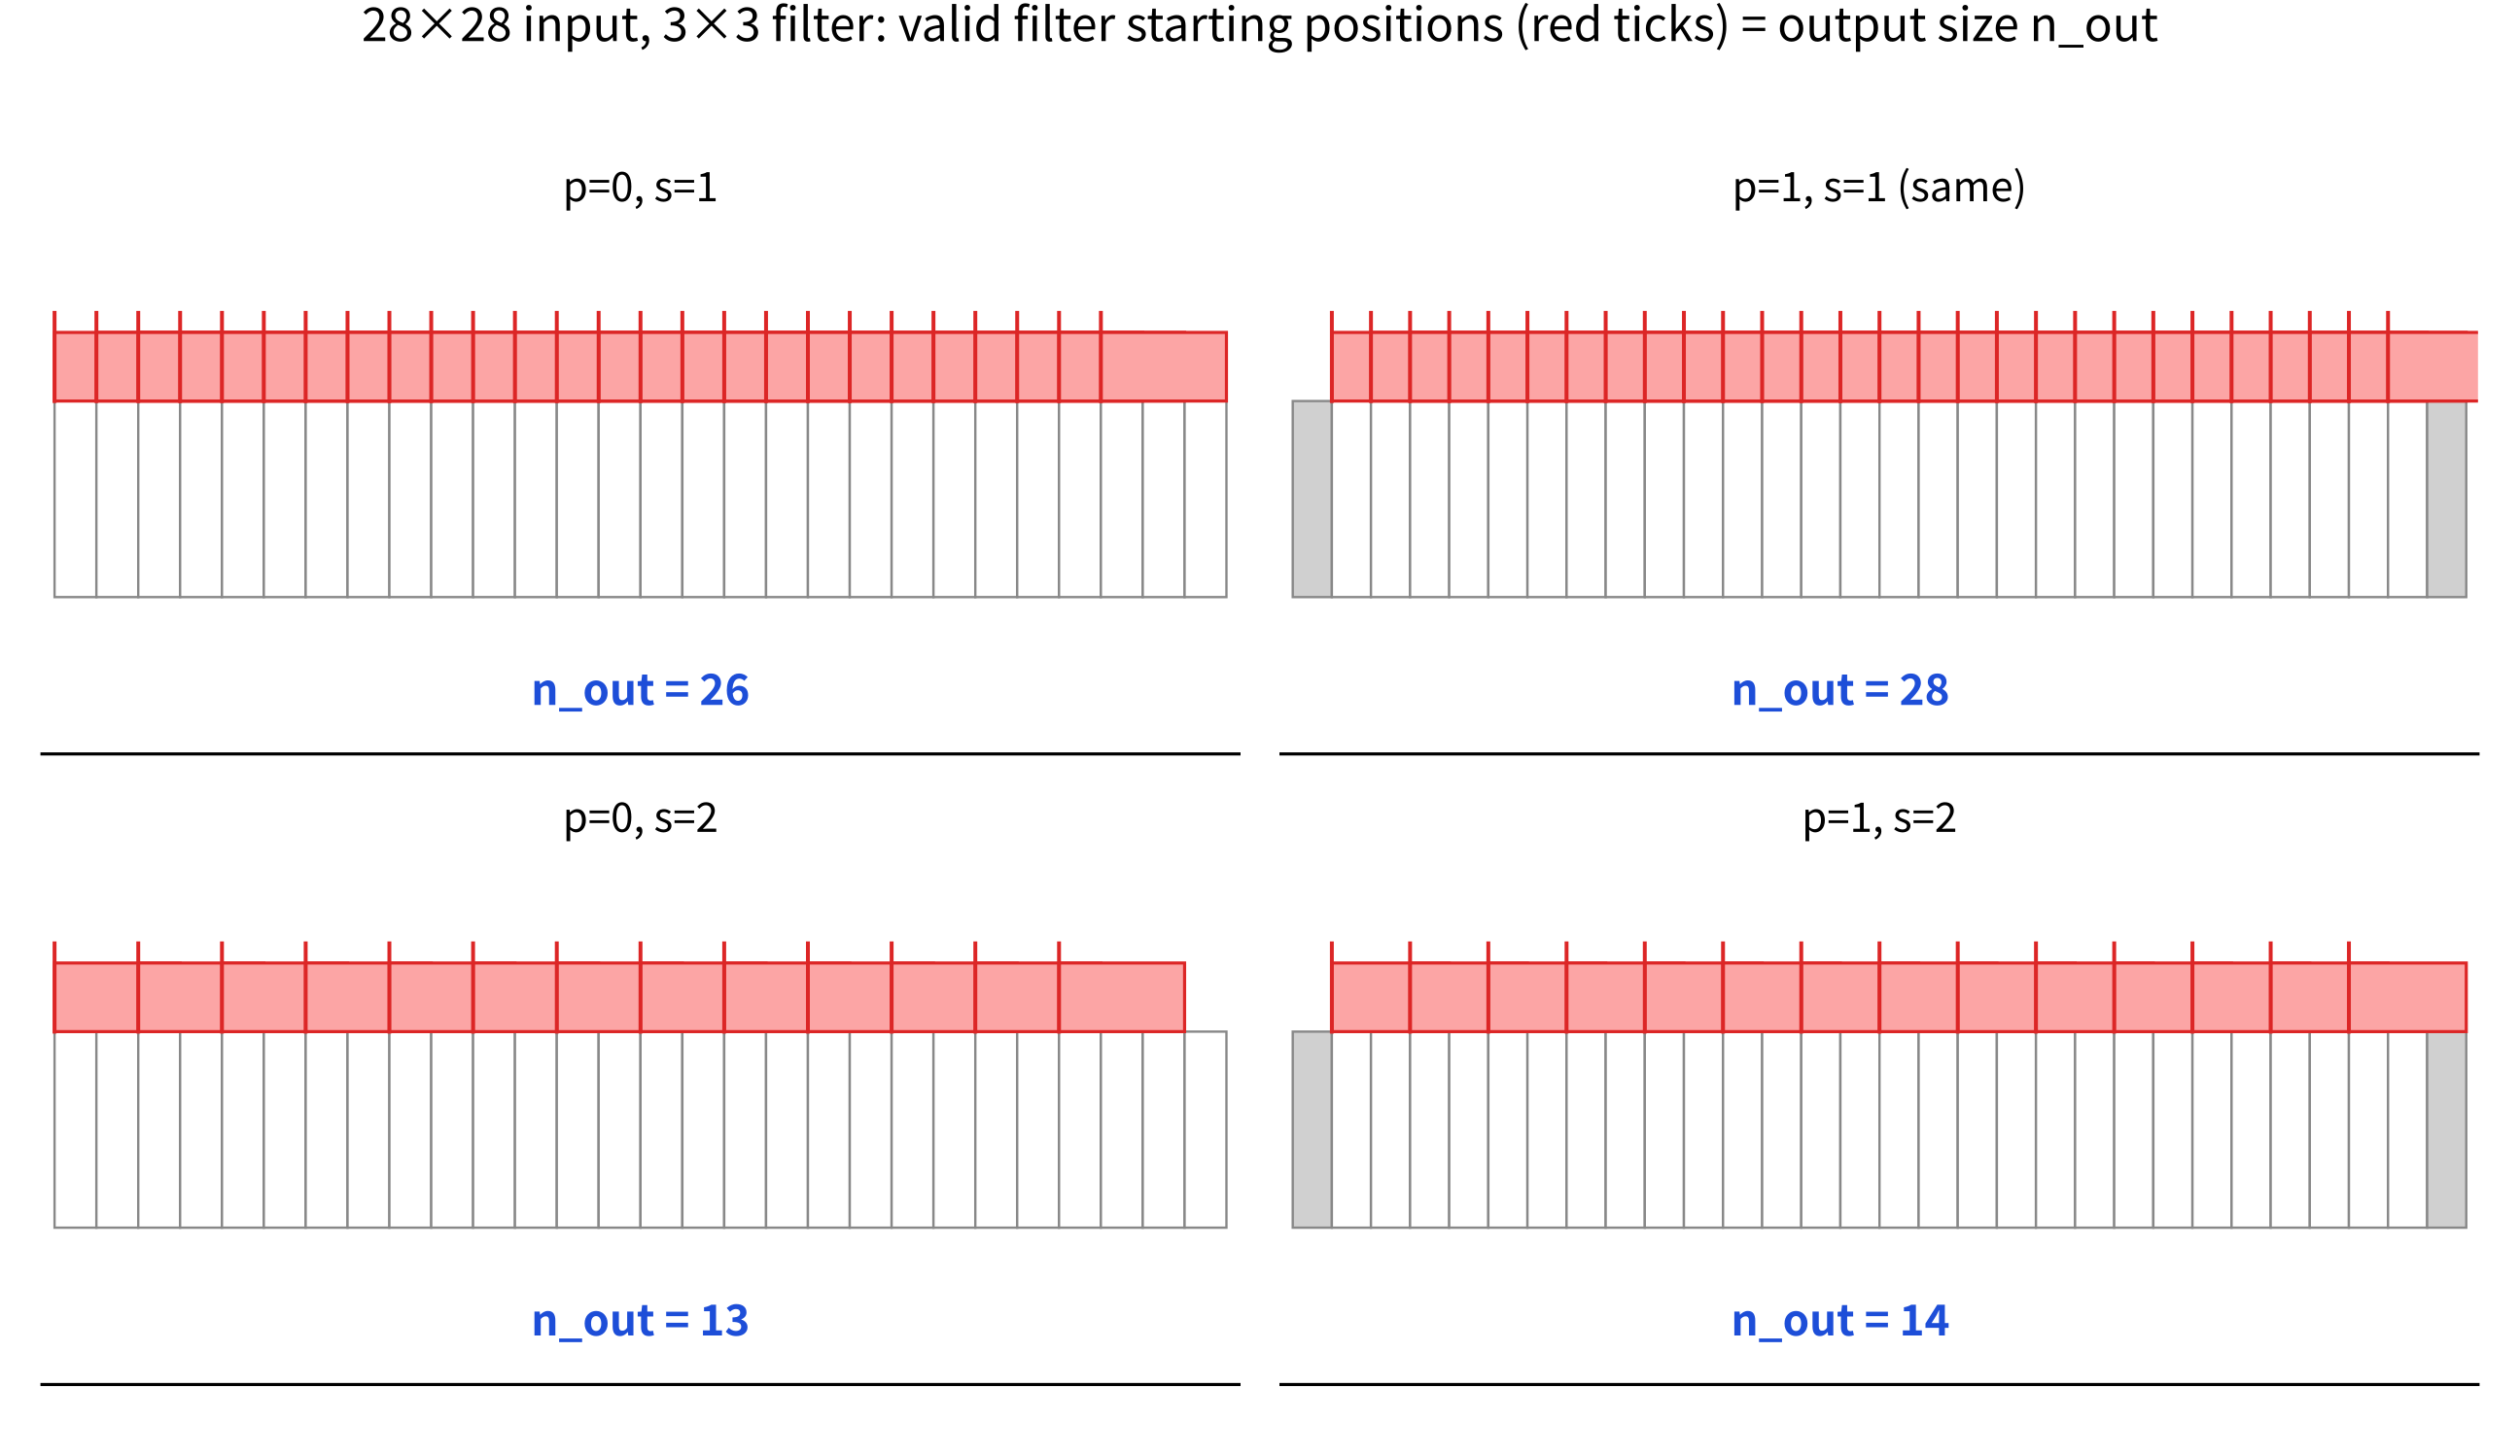
\includegraphics[width=\linewidth]{ch10_1_padding_strides.png}
      \\[0.3em]{\footnotesize 같은 28$\times$28, k=3 을 1D로 줄여
      (p, s) 조합 4가지 --- 회색은 패딩, 각 틱(tick)은 유효한 필터
      시작 위치 하나. \textbf{틱의 개수가 곧 $n_{\text{out}}$}:
      $p{=}0,s{=}1 \to 26$ · $p{=}1,s{=}1 \to 28$ (same) ·
      $p{=}0,s{=}2 \to 13$ · $p{=}1,s{=}2 \to 14$.
      네 숫자 모두 $\lfloor(28+2p-3)/s\rfloor+1$ 로 그대로 계산된다.}
    \end{column}
  \end{columns}
\end{frame}

\begin{frame}{스트라이드 $s=2$가 실제로 하는 일}
  \begin{itemize}
    \item 1D에서 길이를 반으로, 2D에서는 \textbf{가로·세로 둘 다} 반으로
    \item $\Rightarrow$ 공간 \textbf{면적은 1/4}로 줄어든다
    \item 예: 224$\times$224 에 $k{=}3, p{=}1, s{=}2$ 이면
      $n_{\text{out}} = \lfloor(224+2-3)/2\rfloor+1 = \mathbf{112}$
  \end{itemize}
  \vskip0.6em
  \begin{block}{AlexNet(2012)의 첫 합성곱 층}
    정확히 이 설정(224$\to$112)으로 다운샘플링한다.
  \end{block}
  \vskip0.4em
  10.2절에서 2$\times$2 \textbf{풀링}도 면적을 1/4로 줄여주는 것을
  보게 되는데, ``둘 중 무엇을 쓰느냐''는 질문이 생긴다 ---
  이 절 FAQ에서 비교한다.
\end{frame}

\begin{frame}{파라미터 수 계산}
  $C_{\text{in}}$ 개 입력 채널, $C_{\text{out}}$ 개 출력 채널(= 필터 개수),
  필터 $k\times k$ 인 합성곱 층의 파라미터 수(bias 포함):
  \[ \text{params} = (k \times k \times C_{\text{in}} + 1) \times C_{\text{out}} \]
  \begin{itemize}
    \item 예: 32$\times$32$\times$3 이미지, 3$\times$3 필터, 출력 채널 16:
      $(3\times3\times3+1)\times16 = \mathbf{448}$ 개뿐
    \item 같은 입력을 \textbf{완전연결층}(출력 뉴런 32$\times$32$\times$16)에
      연결하려면 \textbf{수백만 개}가 필요하다
  \end{itemize}
  \vskip0.6em
  \begin{center}
  \kq{FLOPs는 ``파라미터 수''와는 \textbf{다른 질문}이다.}
  \end{center}
  \begin{itemize}
    \item 파라미터 수 = ``얼마나 \textbf{많은 숫자를 저장}해야 하는가''
    \item FLOPs = ``\textbf{몇 번의 곱셈-덧셈}을 하는가'' (속도)
  \end{itemize}
\end{frame}

\begin{frame}{FLOPs 공식: $n_{\text{out}}^{\,2}$ 이 곱해진다}
  출력의 한 위치·한 채널을 계산하려면 $k\times k \times C_{\text{in}}$ 번
  곱셈이 필요하고, 이걸 \textbf{모든 출력 위치} $\times$ \textbf{모든 필터}
  로 반복:
  \[ \text{FLOPs} \approx n_{\text{out}}^{\,2} \times C_{\text{out}} \times
     (k \times k \times C_{\text{in}}) \]
  \begin{itemize}
    \item 파라미터 수 공식과 거의 똑같이 생겼지만, \textbf{파라미터 수엔
      없던 $n_{\text{out}}^{\,2}$} 이 곱해진다
    \item 이유: 같은 필터(같은 파라미터)를 \textbf{출력 위치마다 재사용}
      하니 파라미터는 적어도, 계산은 그 위치 수만큼 \textbf{반복}
  \end{itemize}
  \vskip0.5em
  예: 224$\times$224 흑백 ($C_{\text{in}}{=}1$), 3$\times$3 필터 1개,
  p=0, s=1: $n_{\text{out}}=222$
  \[ \text{FLOPs} = 222^2 \times 1 \times 9
     = 49{,}284 \times 9 = 443{,}556 \;\; (\text{약 44만 MAC}) \]
  필터를 64개 ($C_{\text{out}}{=}64$)로 늘리면 \textbf{정확히 64배}
  (약 2,839만 MAC) --- \kb{커널 개수를 늘리면 파라미터 수와 연산량이
  똑같이 정비례}로 늘어난다.
\end{frame}

\begin{frame}{손계산 표: 미니 LeNet 세 층의 비용}
  28$\times$28 흑백을 세 합성곱 층 + 한 풀링으로 줄여가는 작은 네트워크:
  \small
  \begin{tabular}{@{}llrll@{}}
    \toprule
    층 & 연산 & 출력 크기 & 파라미터 & FLOPs \\
    \midrule
    입력 & 28$\times$28$\times$1 & — & — & — \\
    conv 1 & k=3, $C_{\text{out}}{=}4$, p=0, s=1 & 26$\times$26$\times$4
             & 40 & 24,336 \\
    conv 2 & k=3, $C_{\text{in}}{=}4$, $C_{\text{out}}{=}8$, p=0, s=1
             & 24$\times$24$\times$8 & 296 & 165,888 \\
    pool & 2$\times$2 max pooling (s=2) & 12$\times$12$\times$8
             & 0 & (비교 연산 864회) \\
    conv 3 & k=3, $C_{\text{in}}{=}8$, $C_{\text{out}}{=}16$, p=0, s=1
             & 10$\times$10$\times$16 & 1,168 & 115,200 \\
    \textbf{합계} & & 10$\times$10$\times$16 & \textbf{1,504}
             & \textbf{305,424} \\
    \bottomrule
  \end{tabular}
  \vskip0.8em
  {\footnotesize conv 2 FLOPs 직접: $n_{\text{out}}=24$, $24^2=576$ 위치
  $\times 8$ 필터 $\times 9\times4=36$ MAC $= 576\times8\times36
  = 165{,}888$. 실습 노트북 §3에서 numpy로 그대로 재계산.}
\end{frame}

\begin{frame}{표를 읽는 법: ``재고'' vs ``유량'', MLP 비교}
  \begin{enumerate}
    \item \kb{파라미터는 뒤로 갈수록 커지지만}(40$\to$296$\to$1,168)
      \kb{FLOPs 최댓값은 conv 2}(165,888) --- FLOPs는 $n_{\text{out}}^2$ 에
      비례하고 conv 2가 공간적으로 가장 크다(24$\times$24).
      conv 3은 채널 2배지만 공간 1/4(10$\times$10)라 오히려 적다
    \item \kb{풀링은 파라미터 0}, 비용도 곱셈-덧셈이 아니라
      \textbf{비교}(4개 중 최댓값) --- FLOPs 합계에서 무시할 만큼 작음
  \end{enumerate}
  \vskip0.5em
  세 합성곱 층을 \textbf{같은 출력 체적}(10$\times$10$\times$16 $=1{,}600$)
  의 \textbf{완전연결층 하나}(784 입력 $\to$ 1,600 뉴런)로 대체하면:
  파라미터 $784\times1{,}600+1{,}600 = 1{,}256{,}000$
  (합성곱 스택의 \textbf{약 835배}), FLOPs $1{,}254{,}400$
  (\textbf{약 4.1배}).
  \vskip0.4em
  \begin{block}{``재고'' vs ``유량''}
    \textbf{파라미터는 ``재고''}(층당 고정 저장),
    \textbf{FLOPs는 ``유량''}(출력 위치마다 반복되는 계산) ---
    ``한 번에'' 보는 대신 \textbf{작은 패치를 재사용}하는 합성곱이
    \textbf{약 0.12\%의 파라미터, 1/4의 연산}으로 같은 체적의 특징을
    만든다 --- 게다가 \textbf{위치 불변성}이라는 귀납적 편향까지 덤.
    한쪽만 보고 설계하면 안 된다.
  \end{block}
\end{frame}

\begin{frame}{좁아지고 깊어지는 CNN}
  \begin{columns}[T]
    \begin{column}{0.58\textwidth}
      \centering
      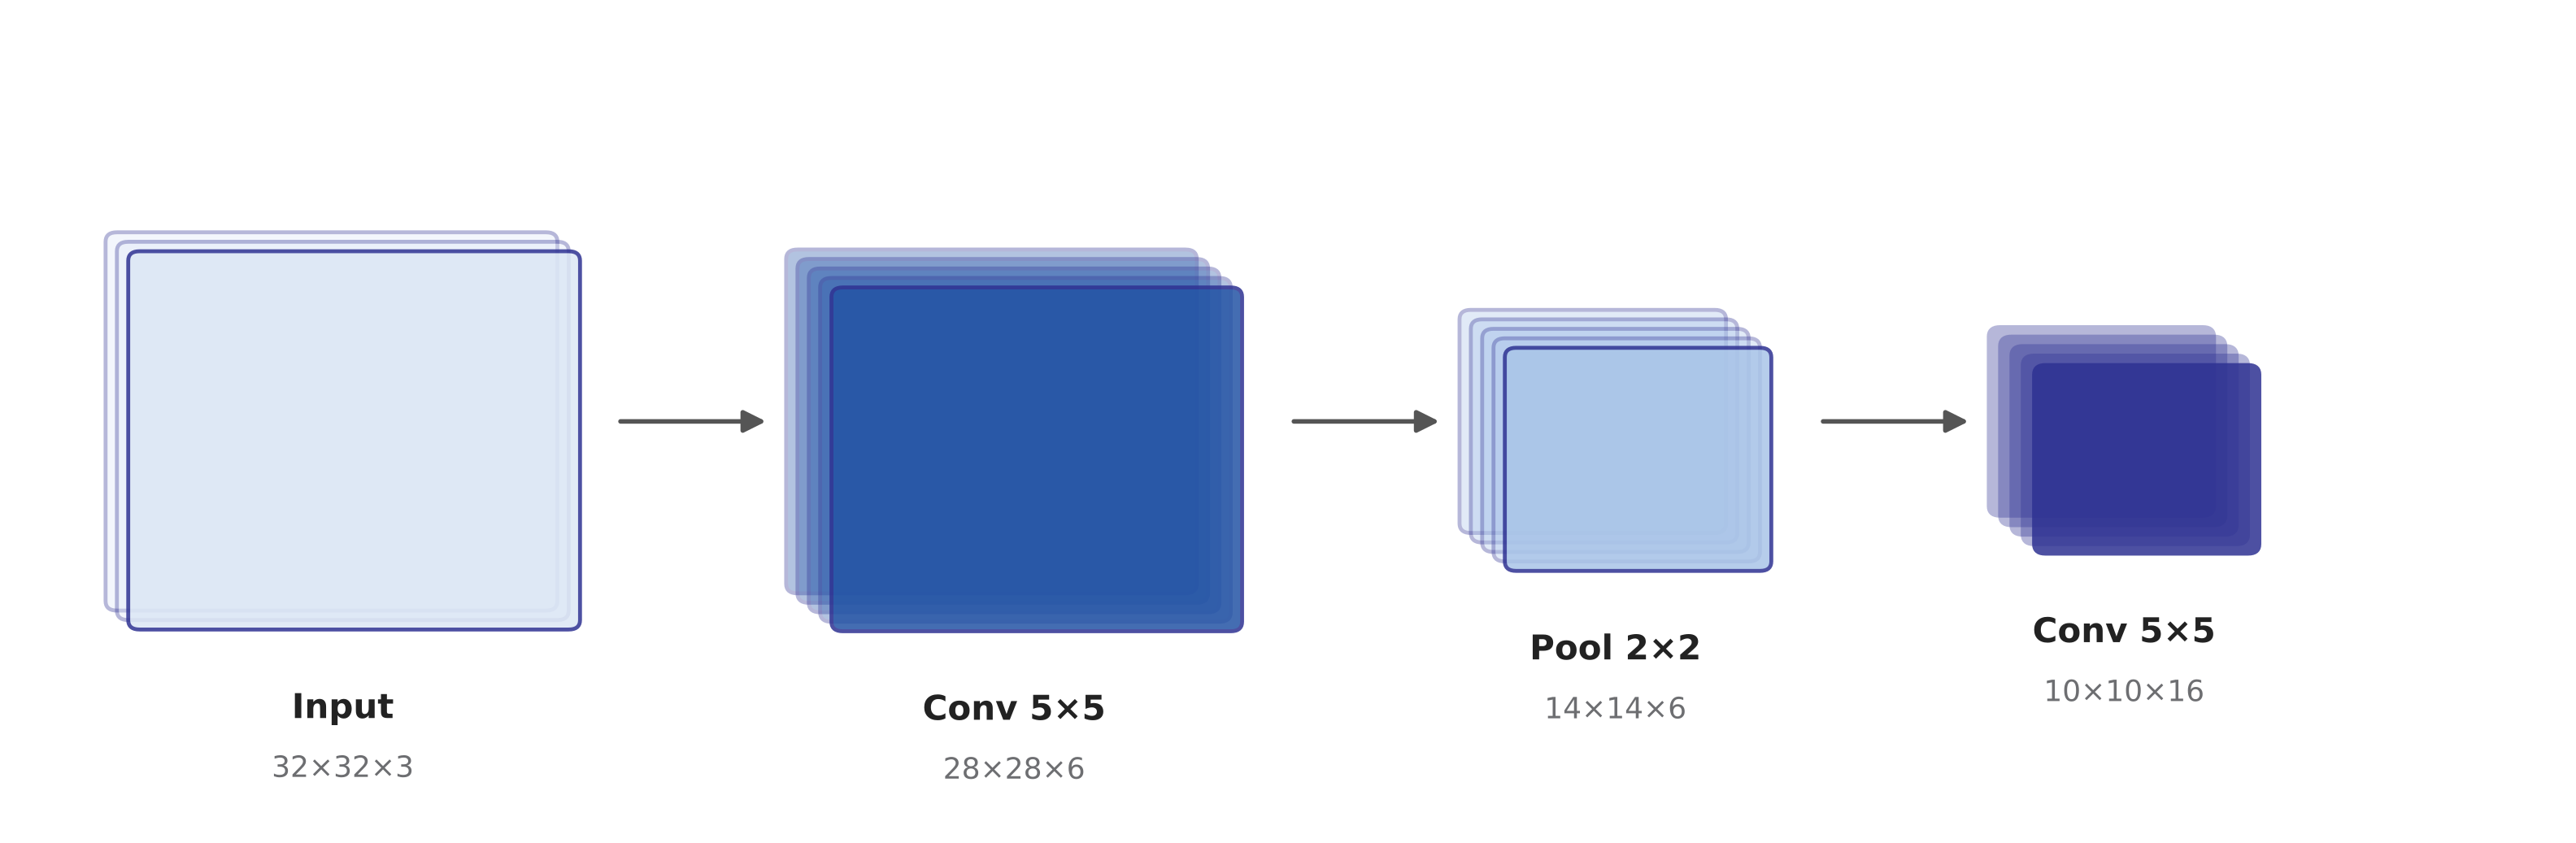
\includegraphics[width=\linewidth]{ch09_cnn_structure.png}
      \\[0.3em]{\footnotesize 합성곱을 거칠 때마다
      \textbf{공간 크기(가로$\times$세로)는 줄고}
      \textbf{채널 수(깊이)는 늘어나}는 모습.}
    \end{column}
    \begin{column}{0.42\textwidth}
      \begin{itemize}
        \item 위 그림의 네트워크:
          32$\times$32$\times$3 $\to$ Conv 5$\times$5 (6ch)
          $\to$ Pool 2$\times$2 $\to$ Conv 5$\times$5 (16ch)
        \item 10.2절 전체를 관통하는
          \textbf{``좁아지고 깊어진다''} 경향의 원형
      \end{itemize}
    \end{column}
  \end{columns}
\end{frame}

\begin{frame}{자주 하는 실수: 공식이 걸리는 두 곳}
  \small
  \begin{columns}[T]
    \begin{column}{0.49\textwidth}
      \kb{실수 1: ``패딩은 출력에 더해지는 거다''}
      \begin{itemize}
        \item $n{=}28, k{=}3, p{=}1, s{=}1$ 의 출력을
          ``$28+2=30$'' 이라고 ---
          패딩 픽셀이 출력을 만든다고 오해
        \item \kb{패딩은 출력 위치를 새로 만들지 않는다} ---
          ``벗어나갈 것 같았던 위치''(필터가 원본 경계를 넘는
          위치)를 \textbf{유효하게 만들어 주는 것}뿐
        \item 출력 = ``패딩된 입력 안에서 필터가 완전히 들어가는
          위치 수'' $= \lfloor(28+2-3)/1\rfloor+1 = 28$
        \item 패딩의 정당한 용도는 \textbf{``same padding으로
          크기를 유지''}, ``출력을 키우는 것''이 아니다
      \end{itemize}
    \end{column}
    \begin{column}{0.49\textwidth}
      \kb{실수 2: ``FLOPs = 파라미터 $\times$ 고정 계수''}
      \begin{itemize}
        \item FC에서는 샘플당 FLOPs $\approx 2\times$파라미터라,
          이 습관을 합성곱에도 적용하기 쉬움
        \item 그러나 \kb{합성곱의 FLOPs/파라미터 비율은
          $n_{\text{out}}^2$ 이며 층마다 다름}
        \item 같은 224$\times$224, 64 출력 채널:
          3$\times$3 = 640 params, $\approx$2,839만 MAC
          vs 1$\times$1 = 128 params, $\approx$321만 MAC
        \item 파라미터 비율 \textbf{5배}인데 FLOPs 비율은
          \textbf{약 8.8배}
      \end{itemize}
    \end{column}
  \end{columns}
  \vskip0.4em
  \kq{연산량을 비교할 때는 ``파라미터 몇 배''가 아니라
  \textbf{공식}으로 직접 계산.}
  {\footnotesize (1$\times$1 합성곱은 공간 크기 그대로 두고
  채널만 선형 결합 --- ``경량으로 채널을 섞는다''는 용도로
  VGG·ResNet 중간층에서 실전에 많이 쓰인다. 10.2에서 다시 만난다.)}
\end{frame}

\begin{frame}[fragile]{실습: 세 공식을 코드 한 페이지로}
  \begin{columns}[T]
    \begin{column}{0.58\textwidth}
\begin{lstlisting}
def out_size(n, k, p=0, s=1):
    return (n + 2*p - k) // s + 1
    # 1D 한 방향의 출력 크기

def conv_cost(n_in, k, c_in, c_out,
              p=0, s=1):
    n_out = out_size(n_in, k, p, s)
    params = (k*k*c_in + 1) * c_out
    flops  = n_out**2 * c_out \
             * (k*k*c_in)
    return n_out, params, flops

print(conv_cost(28, 3, 1, 4))    # (26, 40, 24336)
print(conv_cost(26, 3, 4, 8))    # (24, 296, 165888)
print(conv_cost(12, 3, 8, 16))   # (10, 1168, 115200)
\end{lstlisting}
    \end{column}
    \begin{column}{0.42\textwidth}
      \begin{itemize}
        \item 합계 \textbf{1,504} --- 손계산 표의
          파라미터 합계와 정확히 일치
        \item ``수식 $\to$ 코드 $\to$ 표''가
          하나의 계산을 \textbf{세 번} 확인
        \item 세 공식($n_{\text{out}}$, params, FLOPs)은
          \textbf{독립이 아니라} 같은
          $(n,k,p,s,C_{\text{in}},C_{\text{out}})$ 에서
          나란히 계산되는 \textbf{하나의 패키지}
      \end{itemize}
    \end{column}
  \end{columns}
\end{frame}

\begin{frame}{핵심 공식 한눈에}
  \small
  \begin{tabular}{@{}llp{5.4cm}@{}}
    \toprule
    항목 & 공식 & 무엇을 재나 \\
    \midrule
    출력 크기 & $n_{\text{out}}=\lfloor(n+2p-k)/s\rfloor+1$
        & 합성곱 후 공간 크기 (가로/세로 각각) \\
    파라미터 & $(k^2 C_{\text{in}}+1)\,C_{\text{out}}$
        & 저장해야 할 가중치 수 (bias 포함) \\
    FLOPs & $n_{\text{out}}^{\,2}\,C_{\text{out}}\,k^2 C_{\text{in}}$
        & 곱셈-덧셈 횟수 (출력 위치마다 반복) \\
    관계 & FLOPs $\approx$ (bias 뺀 params) $\times n_{\text{out}}^2$
        & ``재고''와 ``유량''의 차이 \\
    \bottomrule
  \end{tabular}
  \vskip1em
  \begin{center}
  \kq{세 공식은 하나의 패키지다 --- ``재사용''이 만드는 효율의 숫자.}
  \end{center}
\end{frame}

\begin{frame}{FAQ 1·2: 필터 크기와 파라미터 수}
  \begin{block}{Q. 필터 크기는 왜 보통 홀수(3$\times$3, 5$\times$5)?}
    \small
    정확히 \textbf{중심 픽셀이 하나} 있어서 ``어느 픽셀을 중심으로
    보는가''가 자연스럽다. 짝수(2$\times$2)는 중심이 픽셀 사이에
    걸쳐서 대칭 해석이 어렵다. 실전에서는 \textbf{3$\times$3을 여러 겹}
    쌓는 것이 더 널리 쓰인다 --- 3$\times$3 두 개는 5$\times$5 하나와
    \textbf{같은 수용장}을 \textbf{18 vs 25} 파라미터로 만든다.
  \end{block}
  \vskip0.8em
  \begin{block}{Q. 파라미터가 적으면 항상 좋은 건가?}
    \small
    학습이 빠르고 과적합(Ch.\,6) 위험은 줄지만 \textbf{표현력도
    줄어든다} --- Ch.\,4.1의 편향-분산 트레이드오프가 그대로 적용.
    CNN이 이미지에서 유리한 이유는 ``파라미터가 적어서''가 아니라,
    그 적은 파라미터가 \textbf{위치 불변성}이라는 이미지의 실제
    구조에 맞는 \kb{귀납적 편향(inductive bias)} 을 인코딩하고 있기
    때문이다.
  \end{block}
\end{frame}

\begin{frame}{FAQ 3: 스트라이드 2 vs 2$\times$2 풀링}
  둘 다 면적을 1/4로 줄이는데, \textbf{세 가지 차이}:
  \begin{enumerate}
    \item \kb{정보 처리}: max pooling은 4개 중 3개를 \textbf{버리고}
      최댓값 하나만 남김(미분 불가, 정보가 돌이킬 수 없이 사라짐).
      stride-2 합성곱은 각 창 안 $k^2C_{\text{in}}$ 개를
      \textbf{가중치로 합성}(미분 가능, ``다운샘플링 직전에 뭘
      살릴지''가 학습 대상)
    \item \kb{자유도}: 풀링은 창 크기(2$\times$2)와 축소율(1/2)이
      함께 묶여, stride 합성곱은 필터 크기와 스트라이드를
      \textbf{독립적}으로 고를 수 있다(5$\times$5, s=2)
    \item \kb{역사}: LeNet·AlexNet·VGG 시절에는 max pooling이 표준
      다운샘플러, \textbf{ResNet 이후} 고해상도 네트워크에서는
      \textbf{stride-2 합성곱}이 주류 --- 다운샘플링 자체를
      네트워크가 학습
  \end{enumerate}
  {\footnotesize 현대 네트워크는 둘을 섞어 쓰는 경우가 많다.}
\end{frame}

\begin{frame}{FAQ 4·5: FLOPs의 bias, PyTorch 확인}
  \begin{block}{Q. FLOPs 공식에 bias의 ``$+1$''이 없는데?}
    \small
    bias는 출력 위치당 \textbf{한 번만} 더해지는 값 ---
    그 비용 $n_{\text{out}}^2 C_{\text{out}}$ 은 주항 대비
    \textbf{1 차수 낮은 차수 항}(일반 3$\times$3 층에서 약 10\% 미만).
    표준 FLOPs 관례는 곱셈-덧셈(MAC) 수로 세고 bias를 무시.
  \end{block}
  \vskip0.8em
  \begin{block}{Q. PyTorch에서 28$\times$28 입력의 3$\times$3 conv
  출력이 정말 26$\times$26인가?}
    \small
    맞다 --- $\texttt{nn.Conv2d(1, 4, 3)}$(기본 padding=0, stride=1)의
    출력은 26$\times$26, $\texttt{nn.Conv2d(1, 4, 3, padding=1)}$ 는
    28$\times$28. PyTorch의 $\texttt{padding}$ 인자는 이 절 공식의
    \textbf{한 변당 패딩 수 $p$} 그대로(총 $2p$). $p=(k-1)/2$ 의
    same-padding 트릭도 똑같이 동작.
    {\footnotesize (참고: 26$\times$26 에 또 p=0의 3$\times$3을 쓰면
    24$\times$24 --- 짝수/홀수가 층을 지나며 바뀌지만
    ``크기 장부'' 문제일 뿐 오류가 아님.)}
  \end{block}
\end{frame}

\begin{frame}{확인 문제 (10.1): 숫자 네 개}
  \small
  \begin{enumerate}
    \item \kb{출력 크기.} 56$\times$56, k=3, p=1, s=2 $\to$
      $\lfloor(56+2-3)/2\rfloor+1 = \mathbf{28}$.
      (224$\to$112 다운샘플링의 2배 크기 버전.)
    \item \kb{파라미터·FLOPs.} 28$\times$28 ($C_{\text{in}}{=}16$),
      5$\times$5, $C_{\text{out}}{=}32$, p=0, s=1:
      (a) $n_{\text{out}}=24$,
      (b) $(25\times16+1)\times32 = \mathbf{12{,}832}$,
      (c) $24^2\times32\times(25\times16) = \mathbf{7{,}372{,}800}$
    \item \kb{MLP 비교.} 앞 네트워크(1,504 / 305,424)와
      같은 체적 FC(784$\to$1,600) --- FLOPs 비율은 ``4배 안팎''인데
      \textbf{파라미터 비율은 훨씬 큰 이유}를 한 문장으로
    \item \kb{실수 찾기.} ``28$\times$28, k=3, p=1, \textbf{s=2} $\to$
      $(28-3+1)/2 + 2 = 15$'' --- 정답은 \textbf{14}.
      패딩은 스트라이드로 나누기 \textbf{전}에 입력에 더해져야 한다:
      $\lfloor(28+2-3)/2\rfloor+1 = 14$
  \end{enumerate}
\end{frame}

% ============================================================
\section{10.2 풀링과 전형적인 CNN 구조}

\begin{frame}{최대 풀링: 이동에 둔감한 특징}
  합성곱 다음에는 보통 \kb{풀링} 층으로 공간 크기를 줄인다.
  \textbf{최대 풀링(max pooling)}은 $2\times2$ 영역마다
  \textbf{최댓값 하나만} 남긴다.
  \begin{itemize}
    \item 위치가 한두 칸 미세하게 움직여도 같은 최댓값이 뽑힐
      가능성 높음 $\to$ 작은 이동에 \textbf{둔감한}
      (translation-invariant) 특징
    \item 풀링은 \kb{학습 파라미터가 없음} ---
      순수한 \kb{다운샘플링} 연산
  \end{itemize}
  \vskip0.6em
  4$\times$4 특징지도를 1픽셀 오른쪽으로 살짝 옮기면
  \textbf{다음 합성곱 층은 전혀 다른 16개의 숫자}를 보게 된다.
  그런데 2$\times$2 최대풀링을 적용하면 \textbf{두 경우 모두}
  같은 결과:
  \[ \text{maxpool} = \begin{bmatrix} 1 & 3 \\ 1 & 4 \end{bmatrix}
  \qquad (\text{원본과 1픽셀 이동, 동일}) \]
\end{frame}

\begin{frame}{``약간 세로선''은 살아남고, ``정확히 어느 픽셀''은 버려진다}
  네 영역 각각(좌상·우상·좌하·우하)에서 원본의 최대값
  $(1,3,1,4)$ 과 이동 후의 최대값 $(1,3,1,4)$ 이 \textbf{같다}.
  \begin{block}{핵심}
    ``여기에 (대략) 세로선 같은 패턴이 있다''는 정보는 \textbf{살아남고},
    ``정확히 어느 픽셀에''는 정보는 \textbf{버려진다}.
  \end{block}
  \vskip0.6em
  \begin{itemize}
    \item 최대풀링이 이동 불변성을 ``완벽히'' 주진 않는다
      (2픽셀 이상 움직이면 풀링 셀 경계를 건너며 달라질 수 있음)
    \item 하지만 \textbf{한두 픽셀의 미세한 위치 변동}에 대해
      특징지도를 ``부드럽게'' 만들어주는 효과는 확실
  \end{itemize}
\end{frame}

\begin{frame}{평균 풀링과 전역 평균 풀링}
  \begin{columns}[T]
    \begin{column}{0.5\textwidth}
      \kb{평균 풀링(average pooling)} ---
      같은 영역의 \textbf{평균}을 남긴다.
      \begin{itemize}
        \item 최대풀링이 ``이 지역의 \textbf{최대 반응}이 얼마나
          컸는가''를 묻는다면, 평균풀링은 ``\textbf{평균 반응}''
        \item 질감(texture) 같은 \textbf{분포 정보}를 더 잘 유지
      \end{itemize}
      그러나 실전에서는 \textbf{최대풀링이 압도적으로} 널리 쓰인다 ---
      소수 강한 반응이 ``이 특징이 있다''는 \textbf{증거}이므로.
    \end{column}
    \begin{column}{0.5\textwidth}
      \kb{전역 평균 풀링(global average pooling, GAP)} ---
      \textbf{극단}: 채널 전체($h\times w$ 모든 위치)의 평균을
      \textbf{하나만} 남겨 공간 차원을 \textbf{아예 없앰}.
      \begin{itemize}
        \item ``16$\times$16 특징지도를 펼쳐 256개 숫자''가 아니라
          ``이 채널의 \textbf{평균 반응 1개}''
        \item 마지막 \textbf{완전연결층의 파라미터를 대폭 줄이는}
          용도 (아래 VGG16에서)
      \end{itemize}
    \end{column}
  \end{columns}
\end{frame}

\begin{frame}{풀링의 효과: 해상도 대 계산 비용}
  10.1절의 FLOPs 공식을 떠올리면 합성곱 연산량은
  $n_{\text{out}}^{\,2}$ 에 비례했다. $2\times2$ 풀링은 한 번에
  $n$ 을 $n/2$ 로 줄이므로:
  \begin{itemize}
    \item \kb{뒤이어서 오는 모든 합성곱 층의 연산량을 1/4로} 만든다
    \item 특징지도를 \textbf{2회} 풀링 $\to$ 공간 크기 1/4
      (연산량 1/16), \textbf{3회} $\to$ 1/8 (1/64)
  \end{itemize}
  \vskip0.6em
  \begin{block}{왜 대형 CNN은 224$\times$224를 7$\times$7로 줄이는가}
    ``이미지 전체의 맥락''을 판단하려면 공간 해상도가 그 정도면
    충분하고, \textbf{남은 용량을 특징의 수(채널) 쪽에 쓰겠다는}
    설계 선택이다.
  \end{block}
\end{frame}

\begin{frame}[fragile]{실습: 4$\times$4 특징지도를 최대풀링으로}
  10.1절의 $\texttt{conv2d}$ 코드와 같은 스타일로 최대풀링 직접 구현:
  \begin{columns}[T]
    \begin{column}{0.60\textwidth}
\begin{lstlisting}
def max_pool(feature_map, pool_size=2):
    h, w = len(feature_map), \
           len(feature_map[0])
    out_h, out_w = h // pool_size, \
                   w // pool_size
    output = [[0.0] * out_w for _
              in range(out_h)]
    for i in range(out_h):
        for j in range(out_w):
            block = [
                feature_map[
                    i*pool_size+di]
                    [j*pool_size+dj]
                for di in range(pool_size)
                for dj in range(pool_size)]
            output[i][j] = max(block)
    return output

fm = [[1, 0, 2, 1],
      [1, 0, 3, 1],
      [1, 0, 4, 1],
      [1, 0, 2, 1]]
print(max_pool(fm, 2))  # [[1, 3], [1, 4]]
\end{lstlisting}
    \end{column}
    \begin{column}{0.40\textwidth}
      \begin{itemize}
        \item ``원본'' 특징지도를 그대로 넣으면
          $\begin{bmatrix}1&3\\1&4\end{bmatrix}$ ---
          앞 계산과 \textbf{정확히 일치}
        \item 1픽셀 이동 버전도 \textbf{같은 결과}
          --- 둔감함이 코드로
      \end{itemize}
    \end{column}
  \end{columns}
\end{frame}

\begin{frame}{자주 하는 실수: 풀링을 ``특징 추출''로 오해}
  \begin{block}{정리}
    풀링은 \textbf{학습 파라미터가 없는 순수 다운샘플링} 연산이다.
    ``특징을 추출한다''는 표현은 \textbf{합성곱 층의 역할},
    풀링의 역할은 \textbf{이미 학습된} 특징지도를
    (a) 공간 해상도를 줄이고, (b) 미세한 위치 변동에
    둔감하게 만드는 것.
  \end{block}
  \vskip0.6em
  이 구분을 섞으면 두 가지 흔한 설계 실수:
  \begin{itemize}
    \item \kb{풀링을 너무 일찍, 너무 많이}: 첫 합성곱 직후
      2$\times$2 풀링을 하면 아직 ``선분''을 감지하는 단계인데
      해상도를 1/4로 줄여 \textbf{세부 정보를 잃음}. 실무에서는
      \textbf{첫 두$\sim$세 합성곱 층은 풀링 없이}(스트라이드 1) 쌓고,
      채널이 충분히 늘어난 뒤 풀링
    \item \kb{풀링을 ``합성곱의 대안''으로}: 풀링은
      \textbf{합성곱 이후}에 쓰는 연산이지, \textbf{대신}이 아니다.
      ``3$\times$3 합성곱이 비싸니까 2$\times$2 풀링으로 대체''는
      학습하는 가중치를 \textbf{아예 없애버리는 것}
      (스트라이드 2 합성곱은 \textbf{학습 가능한} 다운샘플링이라
      혼용되기도 하지만, 근본적 차이가 ``학습 여부'')
  \end{itemize}
\end{frame}

\begin{frame}{수용장: 뒤쪽 층이 ``보게 되는'' 원본 영역}
  풀링의 공간 축소를 다른 관점에서 보면 \kb{수용장(receptive field)}
  의 \textbf{확대}. 합성곱 한 층은 입력의 $k\times k$ 영역만
  직접 보지만, 출력을 \textbf{또} 합성곱·풀링하면 두 번째 층의
  뉴런 하나가 ``보게 되는'' 원본 영역은 더 넓어진다.
  \vskip0.4em
  각 층의 필터 크기 $k_l$, 스트라이드 $s_l$ 일 때, $l$번째 층
  뉴런의 수용장 크기:
  \[ R_l = R_{l-1} + (k_l - 1)\cdot \prod_{j < l} s_j,
     \qquad R_0 = 1 \]
  \begin{itemize}
    \item 한 층의 뉴런은 직전 층의 뉴런 $k_l$개를 ``보는데'',
      각 뉴런이 이미 원본의 $R_{l-1}$ 픽셀을 대표
    \item 인접 $k_l$개의 수용장을 합치면 겹치는 $(k_l-1)$ 픽셀만
      \textbf{새로} 보이고, 이 확장량이 이전 스트라이드 곱만큼
      \textbf{스케일업}
  \end{itemize}
\end{frame}

\begin{frame}{수용장 손계산 + 풀링이 스케일업하는 기제}
  \small
  \begin{columns}[T]
    \begin{column}{0.48\textwidth}
      입력 32$\times$32 예:
      \begin{tabular}{@{}llrrl@{}}
        \toprule
        층 & 연산 & $k$ & $s$ & $R_l$ \\
        \midrule
        0 & 입력 & — & — & 1 \\
        1 & Conv & 5 & 1 & 1+4$\cdot$1 = \textbf{5} \\
        2 & MaxPool & 2 & 2 & 5+1$\cdot$1 = \textbf{6} \\
        3 & Conv & 5 & 1 & 6+4$\cdot$2 = \textbf{14} \\
        \bottomrule
      \end{tabular}
      \vskip0.6em
      \textbf{단 세 층 만에}, 마지막 합성곱 뉴런은 원본의
      14$\times$14 영역(32$\times$32의 약 19\%)을 ``본다''.
    \end{column}
    \begin{column}{0.52\textwidth}
      \begin{itemize}
        \item 3$\times$3, s=1 만 계속 쌓으면
          $R_l = 1+2l$ 으로 \textbf{선형}
        \item \textbf{풀링(s=2)을 한 번만} 끼워도 그 뒤의
          \textbf{모든 확장이 2배 스케일업}
        \item 10층만 쌓아도 수십 픽셀, 풀링을 섞으면
          \textbf{이미지 전체}가 한 뉴런의 수용장
      \end{itemize}
      \vskip0.5em
      \begin{block}{짝을 이룬다}
        \kb{합성곱}(패턴 감지)이 ``\textbf{무엇을} 보는가''를
        학습하고, \kb{풀링}(수용장 확대·해상도 축소)이
        ``\textbf{얼마나 넓은 시야}로 보게 하는가''를 결정.
      \end{block}
    \end{column}
  \end{columns}
\end{frame}

\begin{frame}{16개 층을 쌓아도: 풀링이 시야를 2배로}
  \begin{columns}[T]
    \begin{column}{0.56\textwidth}
      \centering
      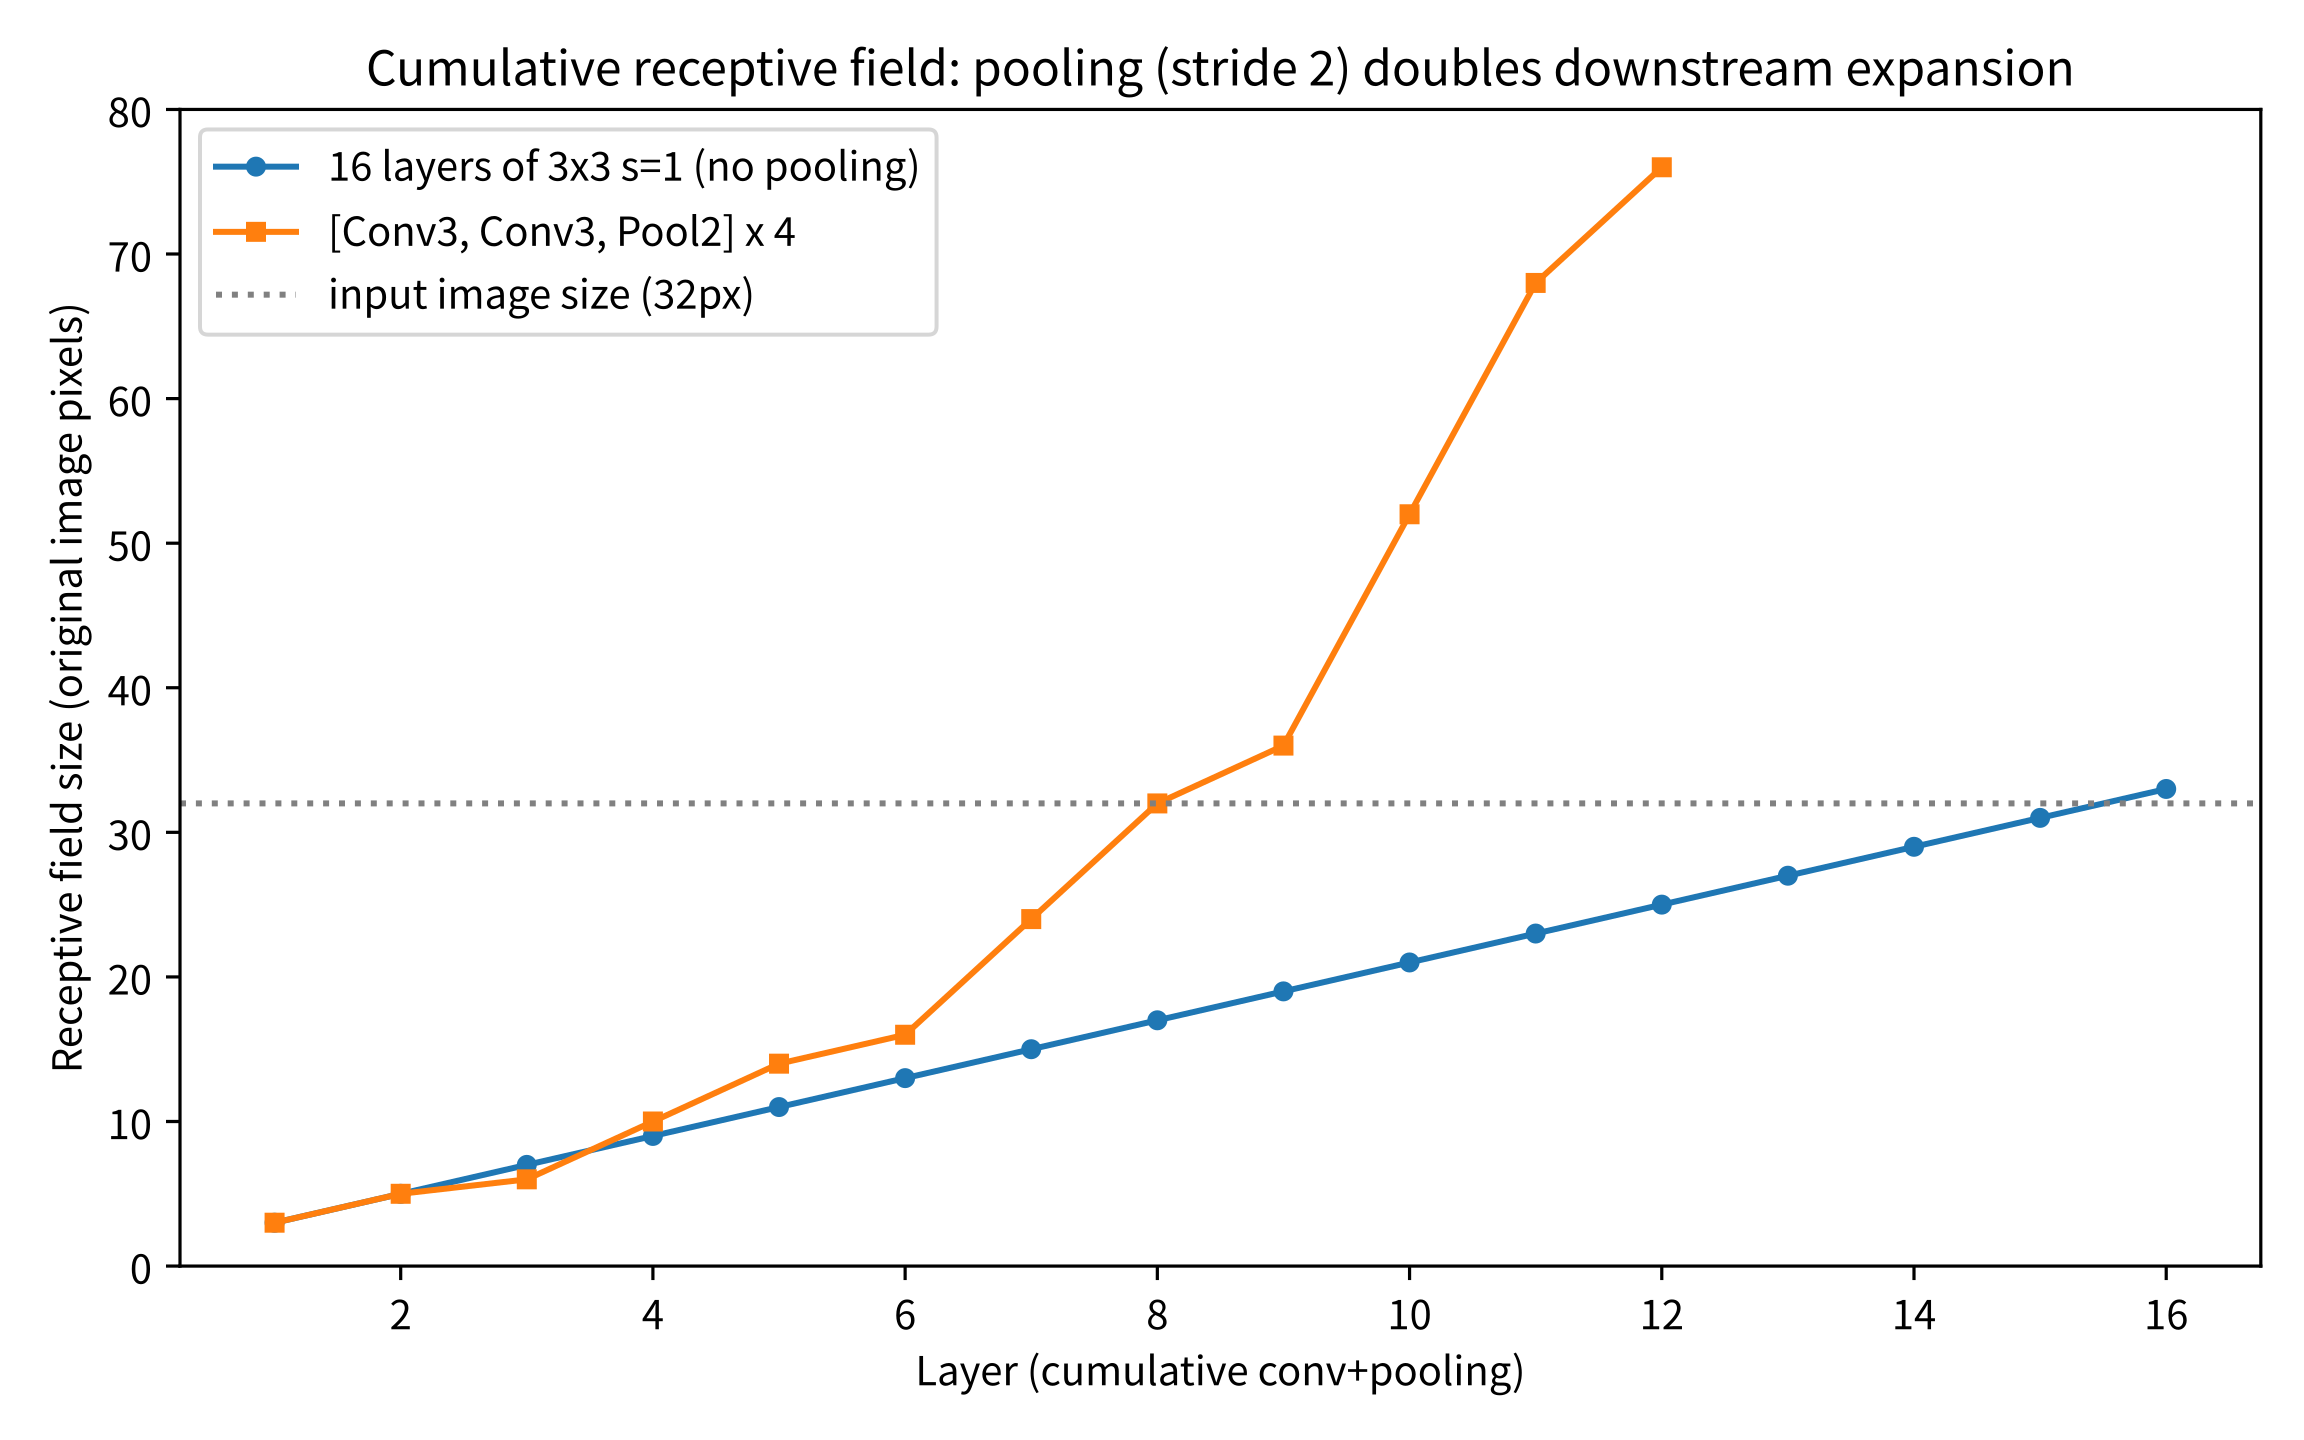
\includegraphics[width=\linewidth]{ch10_2_receptive_field.png}
      \\[0.3em]{\footnotesize 16개 층을 쌓아도 풀링 없이
      스트라이드 1 합성곱만 쌓으면 수용장이 33px(입력 32px과
      비슷)에 그치는 반면, [Conv3, Conv3, Pool2] 블록 4개를
      쌓으면 \textbf{76px} --- 이미지의 2배. 스트라이드 2 풀링
      한 번이 그 뒤의 모든 확장을 2배 스케일업.}
    \end{column}
    \begin{column}{0.44\textwidth}
      \begin{itemize}
        \item Ch.\,4.2 MLP에서 ``은닉층을 쌓을수록 결정경계가
          더 복잡한 형태''라는 관측과 \textbf{같은 원리}
        \item \textbf{얕은 층}은 지역적 패턴(선, 모서리)을,
          \textbf{깊은 층}은 그 지역적 패턴을 \textbf{넓은
          시야에서 조합}한 고수준 특징(눈, 바퀴)을 감지
      \end{itemize}
    \end{column}
  \end{columns}
\end{frame}

\begin{frame}{CNN의 전형적인 구조}
  \[ \underbrace{[\text{합성곱} \to \text{ReLU} \to \text{풀링}]}_{\text{반복}}
  \quad \cdots \quad \to \quad \text{완전연결층 1$\sim$2개} \to \text{분류} \]
  \begin{itemize}
    \item 공간 크기는 \textbf{줄이고}, 채널(특징) 수는 \textbf{늘려}
      가는다가 마지막에 완전연결층을 붙여 분류
    \item \kb{LeNet}(1998, LeCun 등)이 \textbf{손글씨 숫자 인식}에
      처음 이 패턴을 성공적으로 적용한 이래 계층 구조 그대로 유지
    \item 얕은 층 = 선/모서리(저수준), 깊은 층 = 눈/코/바퀴
      (고수준) --- 허블·비셀의 \textbf{단순 세포 $\to$ 복합 세포}
      계층 구조와 같은 원리
  \end{itemize}
\end{frame}

\begin{frame}{LeNet-5 (1998)를 10.1 공식으로 풀기}
  \small
  \begin{tabular}{@{}llrlr@{}}
    \toprule
    층 & 연산 & 출력 크기 & 채널 & 파라미터 \\
    \midrule
    — & 입력 & 32$\times$32 & 1 & — \\
    C1 & 5$\times$5 Conv + sigmoid & 28$\times$28 & 6 & $(25\cdot1+1)\cdot6 = 156$ \\
    S2 & 2$\times$2 MaxPool & 14$\times$14 & 6 & 0 \\
    C3 & 5$\times$5 Conv + sigmoid & 10$\times$10 & 16 & $(25\cdot6+1)\cdot16 = 2{,}416$ \\
    S4 & 2$\times$2 MaxPool & 5$\times$5 & 16 & 0 \\
    C5 & 5$\times$5 Conv + sigmoid & 1$\times$1 & 120 & $(25\cdot16+1)\cdot120 = 48{,}120$ \\
    F6 & 완전연결 (tanh) & — & 84 & $(1\cdot120)\cdot84+84 = 10{,}164$ \\
    OUT & 완전연결 (softmax) & — & 10 & $84\cdot10+10 = 850$ \\
    \midrule
    \multicolumn{4}{@{}l}{\textbf{합계}} & \textbf{$\approx 6.2$만} \\
    \bottomrule
  \end{tabular}
  \vskip0.6em
  각 행은 10.1의 합성곱 공식 $(k^2C_{\text{in}}+1)C_{\text{out}}$ 과
  완전연결 공식 $C_{\text{in}}C_{\text{out}}+C_{\text{out}}$ 을 그대로
  대입(합성곱은 bias 포함, 풀링은 0).
\end{frame}

\begin{frame}{LeNet-5에서 중요한 관찰: ``펼쳐서 FC에 넣기''}
  \begin{itemize}
    \item 구조의 ``형''보다 \textbf{완전연결층이 입력을 어떻게
      받아들이는가}가 중요 --- F6은 C5의 특징지도
      (1$\times$1$\times$120, 즉 120개 숫자)를 \textbf{펼쳐서}
      입력으로 씀
    \item LeNet-5는 C5에서 공간 크기를 이미 1$\times$1로 줄여놨기
      때문에 F6 입력이 120으로 \textbf{작지만} ---
    \item \kb{풀링을 덜 하고 채널을 크게 늘린 네트워크}에서는
      이 ``펼쳐진 벡터''가 \textbf{수만$\sim$수십만 길이}가 되어
      \textbf{완전연결층이 파라미터의 대부분}을 차지
  \end{itemize}
  \vskip0.5em
  이 ``펼쳐서 FC에 넣기''가 비효율이라는 인식이
  10.3절 \textbf{전이학습}(``앞쪽 합성곱은 그대로 쓰고 마지막
  FC 헤드만 재학습'')과 \textbf{전역 평균 풀링}의 동기가 된다.
  \vskip0.3em
  공간 32$\times$32 $\to$ 1$\times$1, 채널 1 $\to$ 120 ---
  ``좁아지고 깊어진다'' 경향의 \textbf{원형}.
\end{frame}

\begin{frame}{AlexNet (2012)과 VGGNet (2014)}
  \begin{itemize}
    \item 1990년대 후반$\sim$2012년 ImageNet 경쟁까지
      ``좁아지고 깊어진다'' 패턴 \textbf{거의 그대로}
    \item \kb{AlexNet}(Krizhevsky, Sutskever, Hinton, 2012):
      ImageNet 우승으로 CNN 시대 개막 ---
      원형은 LeNet과 같은 $[\text{Conv}\to\text{ReLU}\to\text{Pool}]$
      반복, 다만 \textbf{채널}(64, 128, 256, 512)과 \textbf{깊이}를
      크게 늘림
  \end{itemize}
  \vskip0.6em
  \begin{block}{VGGNet(Simonyan \& Zisserman, 2014)의 강력한 관찰}
    \textbf{5$\times$5 필터 하나를 3$\times$3 필터 두 개로 대체}하면,
    \textbf{같은 수용장(5$\times$5)}을 \textbf{더 적은 파라미터}로,
    \textbf{더 비선형으로}(ReLU가 두 번 들어감) 만들 수 있다.
    3$\times$3만 쌓은 16층(VGG16)으로 같은 대회 2위
    (1위는 GoogLeNet, 2014) --- ``\textbf{깊이 자체가 곧 힘}''
    을 널리 퍼뜨림.
  \end{block}
  \vskip0.4em
  \kq{그런데 여기서 문제가 생겼다.}
\end{frame}

\begin{frame}{깊이 열화: 더 깊게 쌓으면 \textbf{나빠진다}}
  2015년, Kaiming He 등(마이크로소프트)이 이상한 현상을 발견:
  CNN을 더 깊게 쌓을수록 성능이 좋아질 줄 알았는데,
  어느 지점을 넘으면 \textbf{오히려 나빠졌다}.
  \begin{itemize}
    \item \kb{과적합이 아니다} --- \textbf{학습 데이터에 대한
      성능조차} 나빠졌다 (training·validation이 \textbf{같이}
      떨어짐)
    \item 층을 더해도 \textbf{그래디언트가 온전히 전달되지 못해}
      깊은 층이 사실상 ``학습이 안 되는'' 문제 ---
      Ch.\,9의 그래디언트 소실이 CNN에서 \textbf{재발}
  \end{itemize}
  \vskip0.5em
  이 현상을 \kb{깊이 열화(degradation)} 라고 부른다:
  ``20층 네트워크는 뒤 10층을 \textbf{항등 함수}로 초기화하면
  앞 10층 네트워크와 \textbf{정확히 동일}''하므로, 이론상 최소한
  10층과 같은 성능을 내야 하는데 실제로는 나빠진다.
  $\Rightarrow$ 원인은 과적합이 아니라 \textbf{최소값 찾기
  최적화 문제}.
\end{frame}

\begin{frame}{깊이 열화 재현: 스킵이 100\%와 50\%를 가른다}
  \begin{columns}[T]
    \begin{column}{0.62\textwidth}
      \centering
      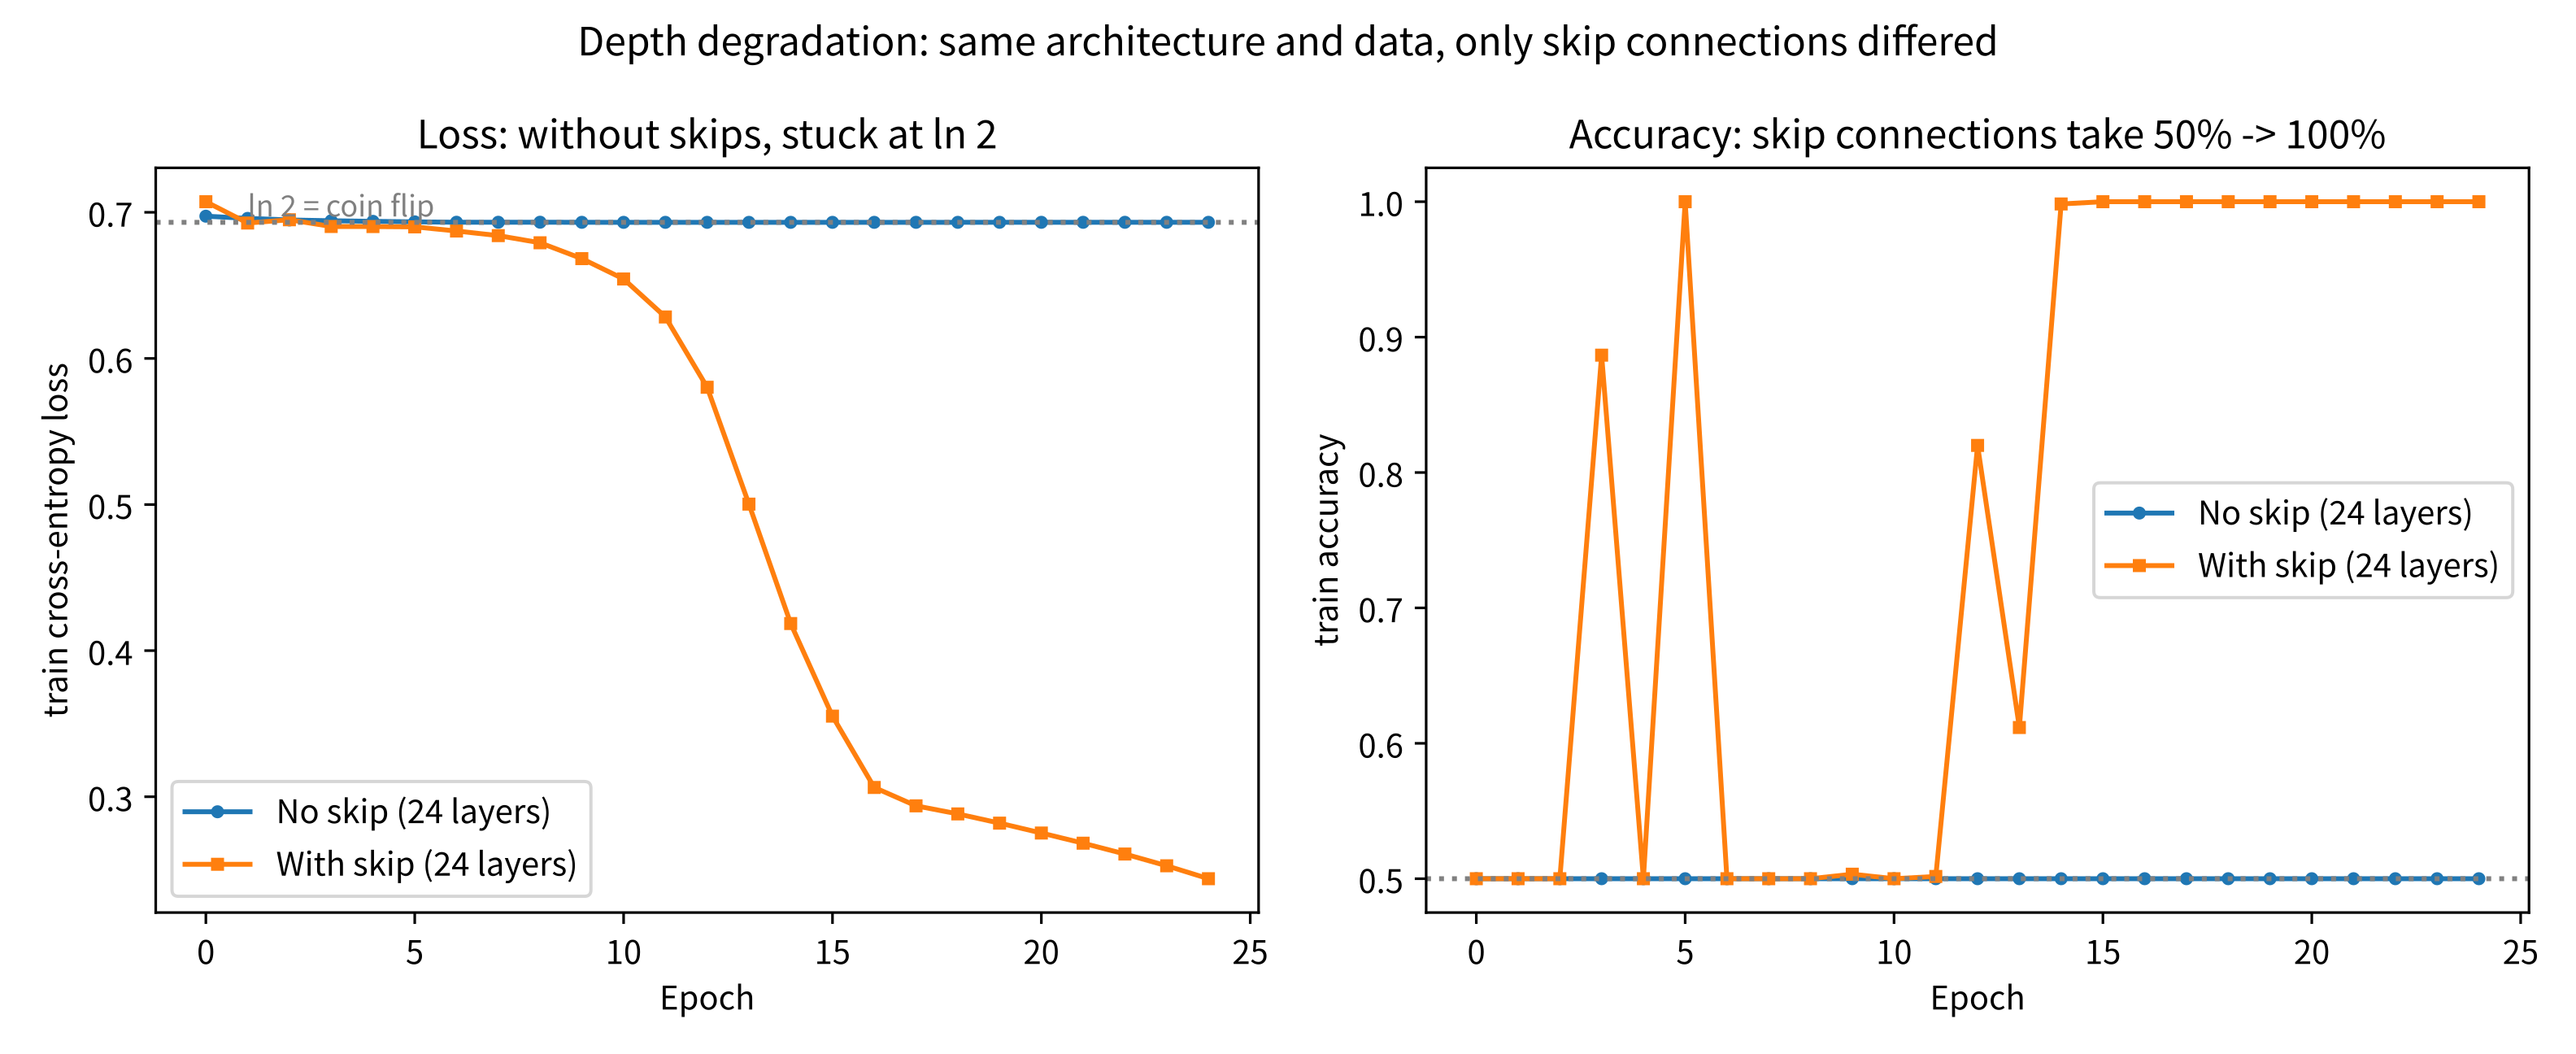
\includegraphics[width=\linewidth]{ch10_2_depth_curves.png}
      \\[0.3em]{\footnotesize 24개 합성곱 층(3$\times$3 Conv-Conv
      블록 12개)을 세로줄/가로줄 데이터로 25 에폭 학습.
      왼쪽: cross-entropy loss --- 스킵 없이는 $\ln2$ 근처에서
      거의 움직임 없음. 오른쪽: train 정확도 --- 스킵이 있는
      버전만 100\%에 도달. 구조·데이터·초기화 시드 모두 같고
      \textbf{스킵 연결만} 달랐다.}
    \end{column}
    \begin{column}{0.38\textwidth}
      \begin{itemize}
        \item \textbf{평범 24층}(스킵 없음):
          loss $\approx 0.693$ ($\ln2$, 동전 던지기),
          train\_acc \textbf{0.500으로 고정}
        \item \textbf{잔차 24층}(스킵 있음):
          15 에폭에 loss 0.355,
          \textbf{25 에폭 내 100\% 도달}
        \item 매우 단순한 분류라 ``학습 못 한다''가
          \textbf{극단적으로} 드러난 예 ---
          ImageNet에서는 점진적으로,
          메커니즘은 같음
      \end{itemize}
    \end{column}
  \end{columns}
\end{frame}

\begin{frame}[fragile]{스킵 연결: $y = F(x) + x$}
  \begin{columns}[T]
    \begin{column}{0.52\textwidth}
      \kb{스킵 연결(skip / residual connection)}은
      그래디언트 \textbf{곱셈 사슬에 지름길}을 낸다 ---
      한 블록의 출력을 $F(x)$ 로 두는 대신,
      \textbf{입력을 그대로 더한} $y=F(x)+x$ 로 정의:
\begin{lstlisting}
def residual_block(x, F):
    # F: 합성곱 층 몇 개로 이루어진
    #    함수 (예: Conv-ReLU-Conv)
    return [F(x)[i] + x[i]
            for i in range(len(x))]
    # F(x) + x
\end{lstlisting}
    \end{column}
    \begin{column}{0.48\textwidth}
      \textbf{왜 그래디언트를 살리는가}(직관):
      $y=F(x)+x$ 를 $x$ 로 미분하면
      \[ \frac{\partial y}{\partial x}
         = \frac{\partial F}{\partial x} + 1 \]
      \begin{itemize}
        \item Ch.\,9의 $\prod_l \sigma'(z_l)\cdot W_l$
          곱셈 사슬에서 $\partial F/\partial x$ 가
          아무리 작아져도(소실),
          \textbf{``$+1$'' 항} 덕분에 그래디언트가
          \textbf{최소 1은 유지}된 채 전달될 길 남음
        \item 입력을 ``건너뛰어'' 뒤쪽 층으로
          \textbf{그대로 흘려보내는 지름길}
      \end{itemize}
    \end{column}
  \end{columns}
  \vskip0.3em
  이 아이디어 덕분에 \textbf{100층이 넘는 CNN도 안정적으로}
  학습할 수 있게 됐고, Ch.\,12의 \textbf{Transformer}에도
  (다른 형태로) 그대로 쓰인다.
\end{frame}

\begin{frame}{``최소한 1''이 정말 성립하는가 --- 수식과 수치}
  $L$개의 잔차 블록을 쌓았을 때, 마지막 출력 $x_L$ 에 대한
  첫 입력 $x_0$ 의 그래디언트는 연쇄법칙으로:
  \[ \frac{\partial x_L}{\partial x_0}
     = \prod_{l=1}^{L} \left( \frac{\partial F_l}{\partial x_{l-1}}
        + 1 \right) \]
  이 곱을 전개하면(각 인자에서 ``1''을 고르거나
  ``$\partial F_l/\partial x_{l-1}$'' 을 고르는 모든 조합의 합)
  정확히 \textbf{한 항}이 ``모든 인자에서 1만 고른'' $= 1$:
  \[ \frac{\partial x_L}{\partial x_0}
     = 1 + \text{(나머지 항들의 합)} \]
  스킵이 없으면 0에 수렴했을 경로에 항상
  \textbf{``1''이라는 바닥}이 깔려 있다. 수치로도 확인:
  무작위 초기화(표준편차 0.1)의 20층 FC에서
  출력에 대한 입력의 그래디언트 노름:
  \begin{itemize}
    \item 스킵 \textbf{없는} 20층: $|dz/dx| \approx 2.5\times10^{-14}$
      (사실상 0 --- 그래디언트 소실)
    \item 스킵 \textbf{있는} 20층: $|dz/dx| \approx 8.2$
      (신호 유지)
  \end{itemize}
  같은 가중치·구조, 스킵 연결만으로 \textbf{약 330조 배}
  ($8.2 / 2.5\times10^{-14} \approx 3\times10^{14}$) 차이.
\end{frame}

\begin{frame}{$F(x)+x$ 의 차원 매칭 + 항등 블록의 시작점}
  \begin{block}{실무: 차원 매칭}
    \small
    더하려면 $F(x)$ 와 $x$ 의 차원(채널 $\times$ 공간)이
    \textbf{정확히 일치}해야 한다. ``채널은 늘고 공간은 줄어든다''
    패턴을 따르면 $F$ 가 64$\to$128 채널, 28$\times$28$\to$14$\times$14
    변환할 때 $x$ 는 그대로 --- \kb{1$\times$1 합성곱}(공간 유지,
    채널만 바꿈)으로 $x$ 의 차원을 맞춰준 뒤 더한다
    (필요하면 2$\times$2 스트라이드 1$\times$1 합성곱으로
    공간도 동시 축소).
  \end{block}
  \vskip0.5em
  \begin{block}{``항등 블록''이 왜 좋은 시작점인가}
    \small
    $F$ 를 \textbf{정규화된(0 근처) 작은 값}으로 초기화하면
    학습 \textbf{시작} 시점에 $F(x)\approx 0$ 이라
    $y\approx x$ --- \textbf{항등 함수로 시작}. ``깊은 네트워크가
    최적의 시작점을 얕은 네트워크의 항등 함수로 가질 수 있다''
    $\Rightarrow$ 학습이 ``0에서 $F(x)$ 를 만들어야 한다''가 아니라
    ``이미 잘 동작하는 항등 함수 위에서 \textbf{잔차만} 미세 조정''.
    ResNet이 ``깊은 망이 왜 어려운가''를 \textbf{표현력} 문제가
    아니라 \textbf{최적화(초기화) 문제}로 재정의한 것.
  \end{block}
\end{frame}

\begin{frame}{배치 정규화: 스킵 연결의 ``공범''}
  ResNet 논문은 스킵 연결과 함께 \kb{배치 정규화(batch
  normalization)}(Ioffe \& Szegedy, 2015)를 결합해 깊은 CNN의
  학습 안정성을 크게 높였다. 합성곱 층 \textbf{사이에} 넣는 층으로,
  각 \textbf{미니배치의 활성값 분포}를 평균 0·분산 1로 표준화한
  뒤, 학습 가능한 $\gamma$(스케일)·$\beta$(오프셋)로 다시
  곱해/더해 ``표준화가 너무 강하지 않게'' 조절:
  \[ \hat{x} = \frac{x - \mu_B}{\sqrt{\sigma_B^2 + \epsilon}},
     \qquad y = \gamma \hat{x} + \beta \]
  \begin{itemize}
    \item $\mu_B, \sigma_B^2$ = 해당 \textbf{미니배치 전체}
      활성값의 평균·분산, $\epsilon$ = 0 나눗셈 방지
      (예: $10^{-5}$)
    \item Ch.\,9.2의 \textbf{초기화 문제를 \textbf{층마다}}
      해결: 100층을 쌓아도 활성값 분산이 층마다 달라지는
      (폭발/소실) 것을 \textbf{학습 중에도} 0·1로 되돌려,
      \textbf{초기화 값에 덜 민감하게} 깊게 쌓을 수 있게
  \end{itemize}
  \vskip0.4em
  ``깊게 쌓기''에 필요한 두 조건 --- 그래디언트가 살아서
  전달되고(스킵), 활성값이 적정 스케일로 유지되고(BN) --- 를
  \textbf{각각 독립적으로} 해결.
  {\footnotesize (10.3에서 BN 통계 처리가 전이학습의
  실전 함정이 되는 것 --- $\mu_B, \sigma_B$ 가 \textbf{학습 시}
  미니배치 기준이라 추론 시에는 \textbf{러닝된} 통계로
  대체해야 함.)}
\end{frame}

\begin{frame}[fragile]{실습: PyTorch $\texttt{SmallCNN}$ + 파라미터 장부}
  세로줄 vs 가로줄(16$\times$16, 잡음 섞임)을 구분하는 아주
  작은 CNN:
  \begin{columns}[T]
    \begin{column}{0.55\textwidth}
\begin{lstlisting}
import torch, torch.nn as nn

class SmallCNN(nn.Module):
    def __init__(self):
        super().__init__()
        self.conv1 = nn.Conv2d(1, 8, 3,
                               padding=1)
        self.conv2 = nn.Conv2d(8, 16, 3,
                               padding=1)
        self.pool = nn.MaxPool2d(2)
        self.fc = nn.Linear(16*4*4, 2)
    def forward(self, x):
        x = self.pool(
            torch.relu(self.conv1(x)))
        x = self.pool(
            torch.relu(self.conv2(x)))
        x = x.view(x.size(0), -1)
        return self.fc(x)
\end{lstlisting}
    \end{column}
    \begin{column}{0.45\textwidth}
      \small
      \begin{tabular}{@{}llrr@{}}
        \toprule
        층 & 연산 & 출력 & 파라미터 \\
        \midrule
        — & 입력 16$\times$16 & 16$\times$16$\times$1 & — \\
        Conv1 & 3$\times$3 + ReLU (same) & 16$\times$16$\times$8 & 80 \\
        Pool1 & 2$\times$2 MaxPool & 8$\times$8$\times$8 & 0 \\
        Conv2 & 3$\times$3 + ReLU (same) & 8$\times$8$\times$16 & 1{,}168 \\
        Pool2 & 2$\times$2 MaxPool & 4$\times$4$\times$16 & 0 \\
        FC & 완전연결 & 2 & 514 \\
        \midrule
        \multicolumn{3}{@{}l}{\textbf{합계}} & \textbf{1{,}762} \\
        \bottomrule
      \end{tabular}
      \vskip0.4em
      {\footnotesize Adam(lr=0.01) + CrossEntropyLoss.
      초기 52\%(동전 던지기) $\to$ 30 에폭 후
      train/val \textbf{100\%}.}
    \end{column}
  \end{columns}
  \vskip0.2em
  {\footnotesize 10.3절에서 재사용할 \textbf{같은 모델}.
  실습 노트북에서는 스킵 연결 있는/없는 두 버전으로
  ``깊이 열화'' 실험을 직접 재현.}
\end{frame}

\begin{frame}{FAQ (10.2)}
  \small
  \begin{itemize}
    \item \textbf{왜 풀링 다음에도 계속 합성곱을 쌓나?} 풀링 하나는
      공간 크기만 절반으로 줄일 뿐, \textbf{패턴의 복잡도는
      높이지 못함}. $[\text{합성곱}\to\text{풀링}]$ 을 반복해야
      뒤쪽 뉴런 하나가 점점 \textbf{넓은 수용장}을 보며,
      그 위에서 더 복잡한 패턴(눈, 바퀴)을 조합.
    \item \textbf{ResNet의 ``$+1$''이 그래디언트 폭발을 일으키나?}
      아니 --- 스킵이 매 블록마다 \textbf{곱이 아니라 덧셈}으로
      기여하므로, Ch.\,9.2의 ``곱이 지수적으로 커지는'' 폭발
      메커니즘과 \textbf{다름}. 그래디언트가 \textbf{여러 경로의 합}으로
      전달돼 오히려 신호를 \textbf{더 고르게} 유지.
    \item \textbf{최대풀링의 ``최댓값 위치'' 정보는?} 최댓값 \textbf{그
      자체}만 남기고 \textbf{어느 픽셀}이었는 정보는 \textbf{버림}
      --- 이게 ``미세 이동에 둔감''한 원리. \textbf{정확한 위치}가
      필요한 문제(탐지)에서는 풀링을 거의 쓰지 않고
      \textbf{스트라이드 2 합성곱}으로 다운샘플링, 또는
      마지막에서 공간 \textbf{복원}(10.3 분할).
      ``위치 보존''과 ``이동 불변성''은 \textbf{트레이드오프}.
    \item \textbf{평균풀링을 쓰는 경우?} \textbf{전역} 평균풀링은
      VGG16·현대 CNN의 마지막 분류층 \textbf{앞}에서 FC 파라미터를
      크게 줄이는 용도로. \textbf{지역} 평균풀링(2$\times$2 평균)도
      ``질감 분포'' 요약에 쓰이지만 최대풀링보다 널리 쓰이지 않음.
    \item \textbf{``깊이 열화''가 과적합이 아닌 근거?} ResNet 논문의
      결정적 실험: \textbf{더 깊은} 망의 \textbf{training} 정확도가
      \textbf{더 얕은} 망의 training 정확도보다 \textbf{나쁨} ---
      과적합은 training이 오르고 validation만 떨어짐. ``모델이
      표현할 수 없어서''가 아니라 \textbf{최적화가 깊게 내려가지
      못해서}.
  \end{itemize}
\end{frame}

\begin{frame}{확인 문제 (10.2)}
  \small
  \begin{enumerate}
    \item \kb{수용장 손 계산.} $k{=}3, s{=}1$ 합성곱 3개
      $\to$ 2$\times$2 maxpool(s=2) $\to$ $k{=}3, s{=}1$ 합성곱 2개.
      마지막 합성곱 뉴런의 수용장:
      $1 \to 3 \to 5 \to 8 \to 14 \to \mathbf{20}$.
      (풀링 한 번이 모든 \textbf{이후} 확장을 2배 스케일업.)
    \item \kb{잔차 그래디언트 항.} $L=3$ 블록에서
      $(A_1+1)(A_2+1)(A_3+1)$ 을 분배법칙으로 완전히 전개하고,
      \textbf{모든 인자에서 ``1''을 고른 항}(= 정확히 1)을
      지목. 이 항이 스킵 없는 $\prod_l A_l$ 에 존재하지 않는
      ``바닥''임을 한 문장으로.
    \item \kb{구조 비교.} LeNet-5($\approx 6.2$만, FC 11,014)와
      $\texttt{SmallCNN}$(1,762)의 파라미터 분포(합성곱 vs FC
      비율)를 비교하고, 10.3의 전이학습이 ``앞쪽 합성곱은
      고정, 마지막 분류층만 재학습''하는 설계가 \textbf{왜
      자연스러운지} LeNet-5 구조(C5가 공간 1$\times$1·채널 120)를
      들어 한 문단으로.
  \end{enumerate}
\end{frame}

% ============================================================
\section{10.3 분류를 넘어서: 탐지, 분할, 전이학습}

\begin{frame}{분류를 넘어서: 두 가지 새 문제}
  지금까지의 CNN은 ``이미지 \textbf{전체}가 어떤 클래스인가''(분류)만
  답했다. 실전 문제는 더 세밀한 답을 요구한다:
  \begin{columns}[T]
    \begin{column}{0.5\textwidth}
      \kb{객체 탐지(Object Detection)}
      \begin{itemize}
        \item ``이미지 안에 사물이 \textbf{어디에}, \textbf{무엇}이
          있는가''
        \item 각 사물의 \textbf{위치}를 사각형
          (bounding box, 4개 좌표)으로, 그 안의 \textbf{클래스}를
          함께 예측
      \end{itemize}
    \end{column}
    \begin{column}{0.5\textwidth}
      \kb{의미론적 분할(Semantic Segmentation)}
      \begin{itemize}
        \item ``\textbf{각 픽셀}이 어떤 클래스에 속하는가''
        \item 입력과 \textbf{동일한 크기}의 출력을 내며 각 픽셀에
          클래스 라벨을 붙임
        \item 자율주행: ``이 픽셀은 도로/보행자/차량''
      \end{itemize}
    \end{column}
  \end{columns}
  \vskip0.6em
  \kq{탐지는 ``\textbf{위치까지 붙은 분류}''다 ---
  분류는 벡터 1개를 내지만, 탐지는 사물 \textbf{마다}
  (클래스, x, y, w, h)를 내야 하고 \textbf{사물의 개수조차 모름}.}
  어려운 부분은 ``무엇을 보는가''(10.2가 이미 잘한다)가 아니라
  ``여러 개, 각기 다른 위치''를 \textbf{한 번의 전진전파}로
  다루는가.
\end{frame}

\begin{frame}{R-CNN (2014): ``후보 $\to$ 특징 $\to$ 판정'' 3단계}
  \begin{columns}[T]
    \begin{column}{0.56\textwidth}
      \centering
      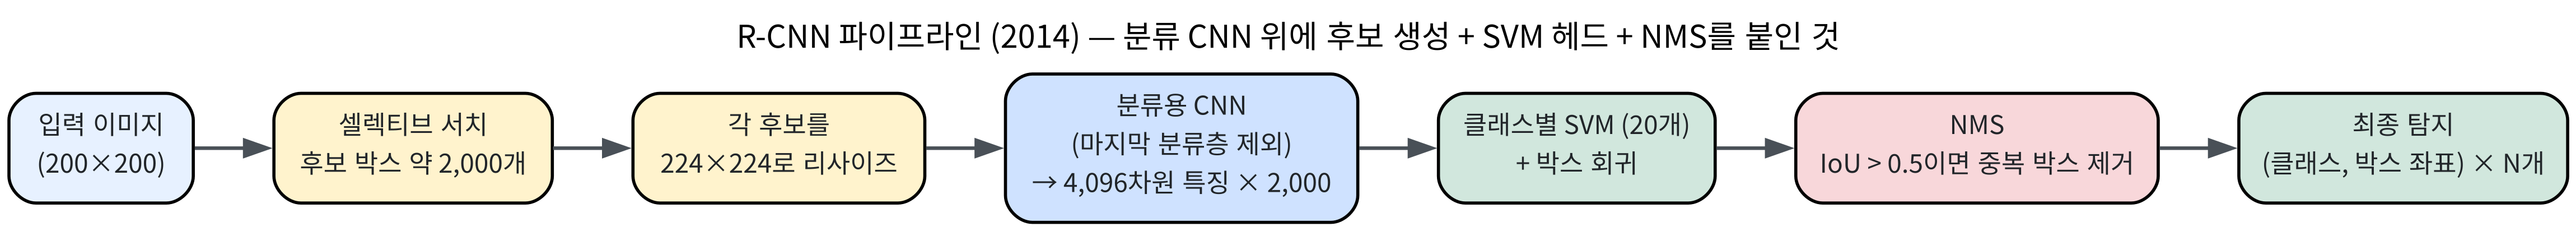
\includegraphics[width=\linewidth]{ch10_3_rcnn_pipeline.png}
      \\[0.3em]{\footnotesize R-CNN 파이프라인 ---
      (1) 셀렉티브 서치로 $\sim$2,000개 후보 박스,
      (2) 각 후보를 224$\times$224로 줄여 CNN을 통과시켜
      4,096차원 특징, (3) 클래스별 SVM + 박스 회귀로 판정,
      (4) IoU 기반 NMS로 중복 박스 제거.}
    \end{column}
    \begin{column}{0.44\textwidth}
      \small
      \begin{enumerate}
        \item \kb{후보 지역}: \textbf{셀렉티브 서치}
          (2012, \textbf{딥러닝이 아닌 기술})가 색·질감이
          비슷한 인접 영역을 합치며 후보 박스
          \textbf{$\sim$2,000개}. 슬라이딩 윈도우(수백만 개)
          대비 ``미리 좁히기''가 통하는 이유: 사물은 실제로
          그렇게 많지 않고 작지도 않은 경우가 대부분
        \item \kb{특징 추출}: 2,000개 후보를 각각
          224$\times$224로 비율만 맞춰 리사이즈하고,
          \textbf{분류용 CNN의 마지막 분류층을 제외한
          부분}을 그대로 통과 --- 각 후보마다 4,096차원
          특징 벡터 1개. \textbf{``분류로 배운 특징
          추출기''를 새 문제에 재사용하는} 순간
        \item \kb{판정}: (a) \textbf{클래스별 SVM 하나씩}
          (Ch.\,5의 SVM --- 20개 클래스면 SVM 20개)로
          ``무엇이'', (b) \textbf{회귀 모델}로 ``정확한
          사물 경계로 미세 조정''. 2,000 후보 $\times$ SVM 20개
          $= 40{,}000$회 판정 --- ``한 특징 벡터는 1번만
          계산해도 4만 번 재사용''되는 또 하나의 파라미터
          재사용
      \end{enumerate}
    \end{column}
  \end{columns}
\end{frame}

\begin{frame}{왜 3단계인가 + 대가: 속도, 그리고 후속 3세대}
  \begin{itemize}
    \item ``여기에 사물이 있을 법한가''(후보) / ``여기에 무슨
      패턴이 있는가''(CNN 특징) / ``도대체 뭘까, 어디까지인가''
      (SVM+회귀) --- \textbf{각 단계에 가장 잘 맞는 도구를 쓰는
      분업}
    \item 대가는 \textbf{속도}: PASCAL VOC 2012 테스트(20,000장)
      1 GPU 약 \textbf{463초} vs 슬라이딩 윈도우 약
      \textbf{605초}(논문 수치, 약 1.3배)로 ``\textbf{느리지만
      정확했다}'' --- 2014년 ImageNet·PASCAL 탐지를 제패
      (전 SOTA 대비 15\%대 mAP 향상)
  \end{itemize}
  \vskip0.4em
  이후 연구 = ``정확도를 유지한 채 \textbf{어떻게 빠르게 할 것인가}'':
  \small
  \begin{tabular}{@{}llp{8.2cm}@{}}
    \toprule
    모델 & 연도 & 속도화 전략 \\
    \midrule
    Fast R-CNN & 2015 & 이미지 \textbf{하나}를 한 번 통과시켜 특징맵을
      만들고, 후보마다 해당 영역의 특징만 \textbf{풀링으로 공유}
      재사용 --- 2,000회 전진전파가 1회로 줄어 \textbf{10배 이상} 빠짐 \\
    Faster R-CNN & 2015 & 후보 추출(셀렉티브 서치) 자체도 학습 가능한
      합성곱 층(\kb{RPN}, Region Proposal Network)으로 ---
      ``2012년 딥러닝 이전 기술''이 마지막 남은 고리 \\
    YOLO & 2016 & 후보도 단계도 없애고, 특징맵의 \textbf{격자 위치마다}
      (클래스, 박스 좌표)를 \textbf{한 번의} 전진전파로 직접 회귀 ---
      탐지를 ``\textbf{회귀 문제로}'' 재정의, 실시간 탐지의 표준 \\
    \bottomrule
  \end{tabular}
  \vskip0.4em
  네 세대 모두 ``\textbf{합성곱 특징 추출기 + 문제마다 다른 출력
  헤드}'' 골격은 그대로 --- 각각 10.1의 \textbf{파라미터 공유},
  Ch.\,9의 \textbf{학습 가능한 구성요소}, 10.2의 \textbf{격자
  특징맵}이 탐지에 적용된 모습.
\end{frame}

\begin{frame}{IoU: 박스의 겹침을 재는 법}
  탐지 모델은 같은 사물에 \textbf{겹치는 박스 여러 개}를 낸다.
  그래서 학습이 \textbf{아닌} 고정 후처리 \kb{NMS(Non-Maximum
  Suppression, 비최대 억제)}가 붙고, 여기서 ``겹기''는
  \kb{IoU(Intersection over Union)}로 잰다:
  \[ \text{IoU}(A, B) = \frac{|A \cap B|}{|A \cup B|}
     = \frac{\text{겹치는 면적}}{\text{합쳐진(겹침 한 번만) 면적}} \]
  \begin{itemize}
    \item $[0,1]$ 에 있고 \textbf{1이면 완전 일치}
    \item Ch.\,3의 \kb{재카드 지수}(Jaccard index)가
      \textbf{면적 버전}으로 ``박스 두 개의 비슷함''을 재는 것
  \end{itemize}
  \vskip0.4em
  \textbf{손으로}: $A=[0,0,10,10]$, $B=[1,1,11,11]$ ---
  교집합 $[1,1,10,10]$ $\to$ 면적 $9\times9=81$,
  합집합 $100+100-81=119$.
  \[ \text{IoU} = 81/119 \approx \mathbf{0.68} \]
  \textbf{왜 IoU인가} --- ``교집합/작은 박스''나 ``박스 중심거리''가
  안 되는 이유는 \kb{스케일 불변성}: 중심거리는 박스가 크면 같은
  겹기라도 ``멀어'' 보이고, 교집합/합집합 비율은 박스를 함께
  키우면(스케일) \textbf{변하지 않음}.
  {\footnotesize 탐지 \textbf{훈련 라벨링}에서도 쓰인다 ---
  예측 박스가 정답과 IoU $\ge 0.5$면 ``탐지 성공'' 정밀도
  평가 규칙이 PASCAL VOC·COCO \textbf{표준}. 같은 함수가
  학습·평가 양쪽에 들어가는 셈.}
\end{frame}

\begin{frame}{NMS를 한 번 따라가보자}
  1. 모든 (박스, 점수)를 \textbf{점수 내림차순} 정렬
  2. 가장 점수 높은 박스를 \textbf{보관}하고, 그것과 겹기가
     임계값(보통 $0.5$)을 넘는 모든 박스를 \textbf{제거}
  3. 남은 박스에서 2를 반복
  \small
  \begin{tabular}{@{}llc@{}}
    \toprule
    박스 & 좌표 $[x_0,y_0,x_1,y_1]$ & 점수 \\
    \midrule
    A & $[0,0,10,10]$ & 0.90 \\
    B & $[1,1,11,11]$ & 0.80 \\
    C & $[20,0,30,10]$ & 0.75 \\
    D & $[21,1,31,11]$ & 0.60 \\
    \bottomrule
  \end{tabular}
  \vskip0.6em
  \begin{columns}[T]
    \begin{column}{0.46\textwidth}
      \begin{itemize}
        \item \textbf{A}(0.90) 먼저 보관
        \item B와 IoU \textbf{0.68 $>$ 0.5} $\to$ \textbf{제거}
        \item 남은 \textbf{C}(0.75) 보관, D와 IoU 0.68
          $\to$ \textbf{제거}
        \item \textbf{결과: A와 C만 남음} --- 4개 박스에서
          사물 2개. A,B 쌍과 C,D 쌍의 IoU가 \textbf{같은 값
          0.68}을 두 번 씀으로써 ``제거 기준은 점수가
          아닌 \textbf{겹기}''임을 보임
      \end{itemize}
    \end{column}
    \begin{column}{0.54\textwidth}
      \centering
      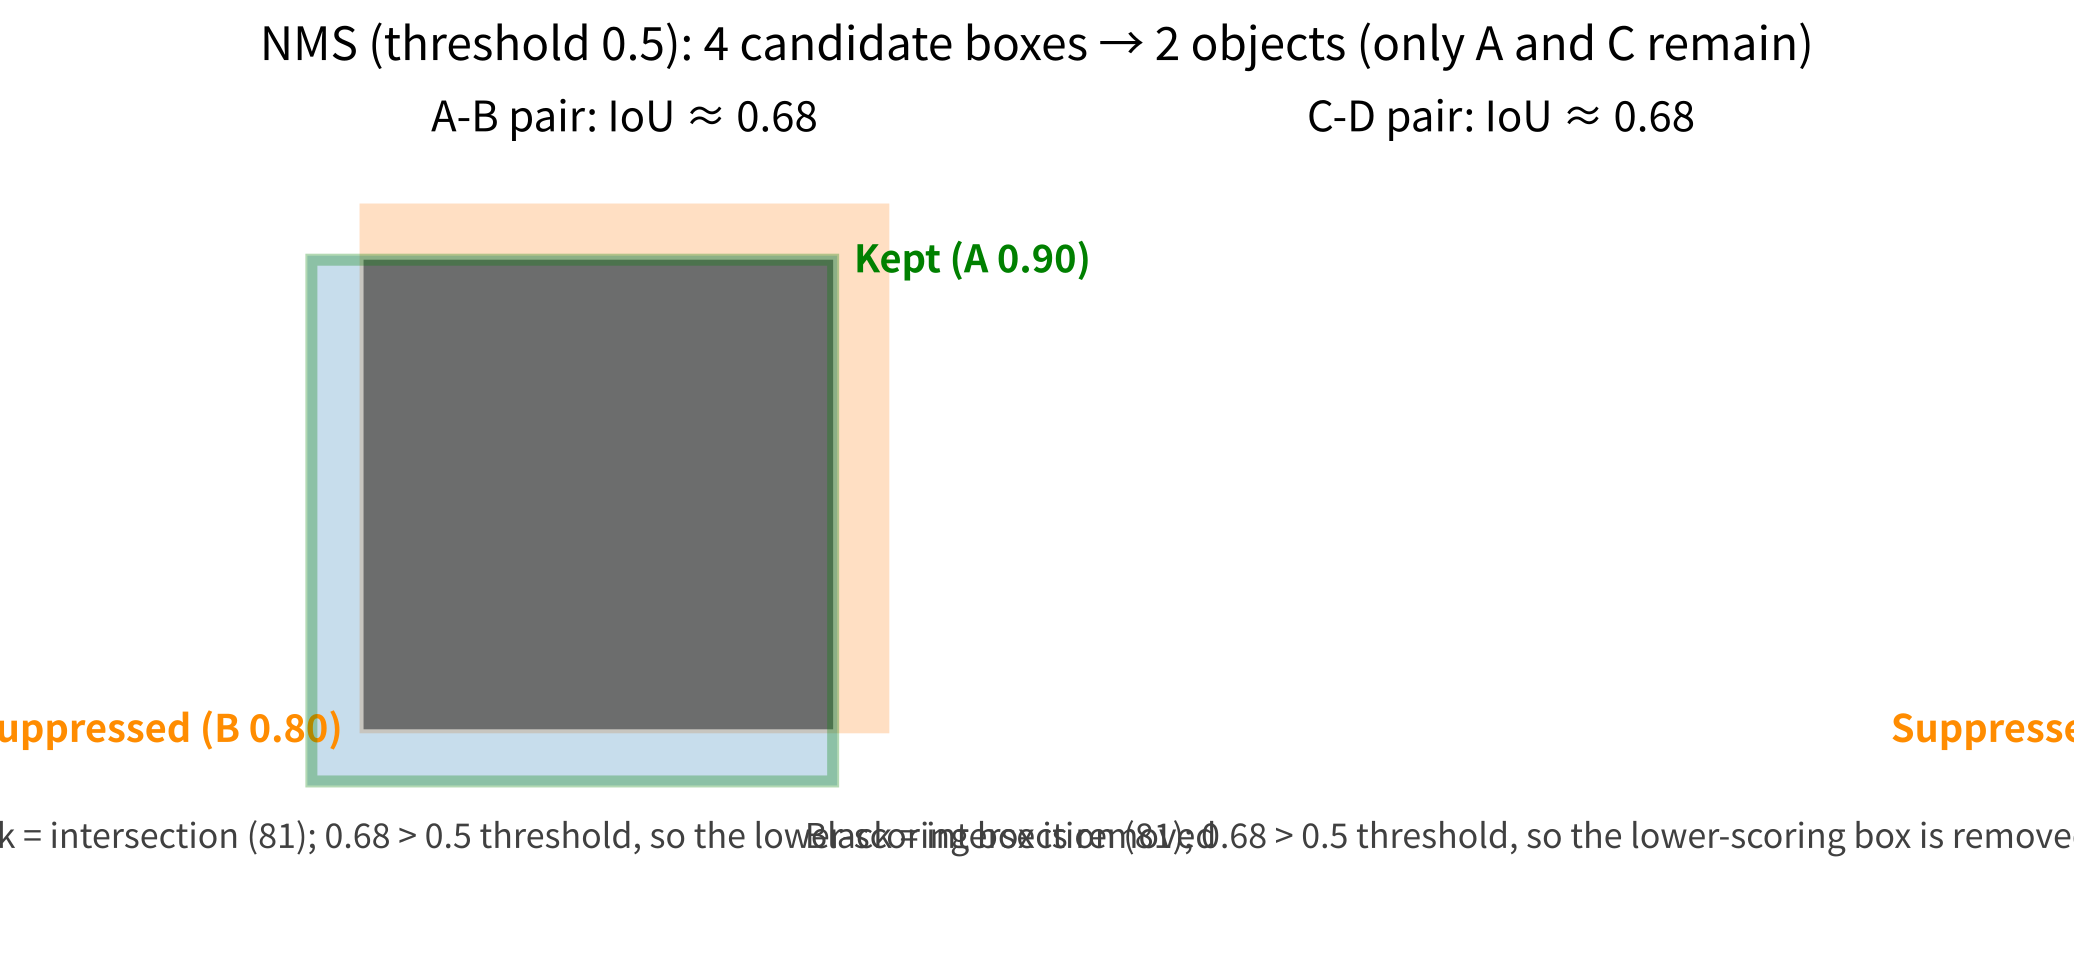
\includegraphics[width=\linewidth]{ch10_3_iou_nms.png}
      \\[0.3em]{\footnotesize 4개 박스 중 NMS(임계값 0.5)가
      A와 C를 남기고 B, D를 제거 --- A와 B의 교집합(검정)이
      합집합의 0.68을 차지해 B가 억제되는 것.}
    \end{column}
  \end{columns}
  \vskip0.3em
  \textbf{임계값 0.5는 왜인가} --- ``맞는 값''이 아니라
  \textbf{조율 대상}: 0.7로 올리면 같은 사물에 박스 두 개가
  남을 수 있고(더블 카운팅), 0.2로 낮추면 서로 다른 사물이
  살짝만 겹쳐도 하나가 통째로 사라진다.
  \textbf{NMS는 왜 학습되지 않는가} --- 10.2 풀링과 같은
  논리: ``점수 높은 쪽을 살리고 겹치는 쪽을 버린다''는
  \textbf{보편 규칙}이라 학습 가능한 파라미터를 붙일 이유가
  없고 라벨도 ``이 박스가 중복이다''로 주어지지 않는다 ---
  \textbf{고정 규칙이 가장 일반화}된다. 파이프라인의 모든
  부위가 미분 가능해야 하는 것은 아니다.
\end{frame}

\begin{frame}{분할: ``격자 위치마다 붙은 분류기''}
  10.2의 분류 네트워크를 끝까지 펼쳐보자 --- VGG 계열처럼
  224$\times$224 입력이 2$\times$2 최대풀링을 \textbf{5번} 거치면
  공간 크기는 $224/2^5 = 7$ 로 줄고, 마지막 합성곱 층의 출력은
  7$\times$7 \kb{격자}(채널 512개). \textbf{분류 헤드}란 그
  격자를 \textbf{펼쳐서} 1,000개 클래스 점수 하나로 모으는 층일
  뿐이다.
  \vskip0.5em
  \begin{block}{의미론적 분할 헤드}
    1개의 헤드 대신, \textbf{49개의 격자 위치마다 ``클래스 1,000개''
    출력을 \textbf{공유 가중치}로 붙인다} --- 마지막 층을
    ``512$\to$1,000 선형층''이 아니라 \textbf{출력 채널 1,000개
    의 1$\times$1 합성곱}으로 바꾸면, 격자 \textbf{각 위치}에서
    512개 특징을 1,000개 클래스 점수로 변환하고 그 가중치는
    49개 위치가 \textbf{공유}(1$\times$1 합성곱이 ``위치당
    분류기'' --- 10.1 FAQ의 ``채널만 선형 결합''). 파라미터는
    $512\times1{,}000+1{,}000$ \textbf{하나분}만 추가되지만,
    답의 형태가 ``벡터 1개''에서 \textbf{7$\times$7 클래스 지도}로
    바뀜.
  \end{block}
  {\footnotesize ``각 픽셀''이 아니라 7$\times$7 격자점인 이유:
  풀링이 공간 정보를 반으로 줄인 5번의 결과 --- 실제 분할
  모델은 풀링을 줄이고 U-Net처럼 해상도를 \textbf{되살리는}
  구조를 쓴다.}
\end{frame}

\begin{frame}{왜 공유가 올바른 편향인가 + U-Net}
  \begin{itemize}
    \item ``이 픽셀이 도로인가''의 정답은 이미지 좌상단이었든
      우하단이었든 \textbf{같은 법칙}으로 결정됨 ---
      10.1에서 ``고양이가 어디에 있든 같은 고양이''라
      \textbf{합성곱}이 위치마다 가중치를 공유한다면, 분할에서는
      ``도로인지 아닌지의 판단법이 어디에서든 같다''라
      \textbf{헤드}가 위치를 공유하는 것 --- 합성곱의 \textbf{재사용
      원리가 파이프라인의 다른 위치}에서 다시 등장
  \end{itemize}
  \vskip0.5em
  \kb{해상도 복원: U-Net}(Ronneberger 등, 2015) ---
  ``7$\times$7 격자 예측을 224$\times$224 원본으로 되돌린다''는
  것은 공간 크기를 5번 \textbf{더블업}(업샘플링)하는 문제,
  \textbf{풀링의 역방향}. ``줄여가는'' \textbf{코더}(encoder) 끝에
  업샘플링으로 ``늘려가는'' \textbf{디코더}(decoder)를
  \textbf{대칭}으로 붙여 \textbf{U자} 형태.
  \begin{itemize}
    \item 디코더만으로는 \textbf{어디가} 도로인지(정확한 경계)를
      되찾기 어려움 --- 위치 정보는 풀링에 이미 \textbf{버려짐}
    \item 해결책은 10.2의 \kb{스킵 연결} --- 코더의
      \textbf{초기 층}(위치 정보가 아직 살아 있는 층)의
      특징맵을 디코더의 \textbf{해당 레벨}에 \textbf{그대로
      건너뛰어 더함}
  \end{itemize}
  \vskip0.3em
  ResNet이 스킵 연결로 \textbf{깊이}를 쌓을 수 있게 했다면,
  U-Net은 스킵 연결로 \textbf{해상도}를 되찾은 셈.
  U-Net이 \textbf{의료 영상 분할}(병리 슬라이드, 초음파)의
  표준인 이유: ``\textbf{몇십 장의 라벨만으로도} 쓸만하게
  학습된다'' --- 전이학습·소데이터 이야기와 정확히 겹치는 지점.
\end{frame}

\begin{frame}{전이학습: 처음부터 다시 배우지 않는다}
  대규모 데이터(ImageNet, 수백만 장)로 \textbf{미리 학습된
  CNN의 앞쪽 층}들은 선/모서리/질감 같은 \textbf{아주 범용적인}
  패턴을 감지하도록 학습돼 있다 --- ``고양이를 구분하는
  능력''이 아니라 \textbf{``이미지를 보는 능력''} 자체에 가깝다.
  \kb{전이학습(Transfer Learning)}은 이 사전학습된 앞쪽
  층을 \textbf{그대로 재사용}하고, 마지막 몇 층만 새 문제에 맞게
  다시 학습시킨다:
  \begin{columns}[T]
    \begin{column}{0.5\textwidth}
      \kb{특징 추출(feature extraction)}
      \begin{itemize}
        \item 사전학습된 층의 가중치를 \textbf{전부 고정
          (freeze)}, \textbf{마지막 분류층만} 새로 학습
        \item \textbf{데이터가 적을 때} 특히 유리 ---
          새로 학습할 파라미터가 훨씬 적기 때문
      \end{itemize}
    \end{column}
    \begin{column}{0.5\textwidth}
      \kb{미세조정(fine-tuning)}
      \begin{itemize}
        \item 사전학습된 가중치를 \textbf{학습의 시작점}으로만
          쓰고, 전체(또는 뒤쪽 일부) 층을 \textbf{낮은 학습률}로
          계속 학습
        \item \textbf{새 데이터가 어느 정도 있을 때} 특징 추출보다
          더 좋은 성능
      \end{itemize}
    \end{column}
  \end{columns}
\end{frame}

\begin{frame}{``앞쪽 층은 범용하다''는 말의 첫 증거}
  \begin{itemize}
    \item 추측이 아니라 \textbf{보여준 것} --- AlexNet 논문
      (Krizhevsky 등, 2012)이 학습된 \textbf{첫 합성곱 층의
      필터를 그림으로 인쇄}했고, 거기서는 방향/색 대비를
      감지하는 \textbf{Gabor 같은 필터}들이 늘어섬
    \item 장 머리에서 허블·비셀이 고양이 시각피질에서 본
      \textbf{단순 세포의 수용장과 동일한 종류}의 패턴
    \item ImageNet 1,000개 클래스를 구분하기 위해 학습된
      네트워크의 첫 층이 ``고양이 특화''가 아니라
      \textbf{``모서리 감지''}에 쓰였다는 뜻
  \end{itemize}
  \vskip0.5em
  \begin{block}{전이학습이 이용하는 비대칭}
    층이 깊어질수록 특징이 눈·바퀴·사물 부분으로
    ``사물화''되는 계층 구조(10.2) 때문에,
    \textbf{앞으로 갈수록 재사용 가치가 높다} ---
    \textbf{앞쪽 = 범용, 뒤쪽 = 특화}.
  \end{block}
\end{frame}

\begin{frame}{같은 작업에서 세 팔(arm) 비교}
  10.2의 $\texttt{SmallCNN}$(세로줄/가로줄 분류) 위에서 ---
  동일 아키텍처·동일 데이터(300 학습/200 검증)·동일 30 에폭,
  \textbf{다만 어느 층이 갱신되는가}만 바꿈:
  \small
  \begin{tabular}{@{}lll@{}}
    \toprule
    팔 & 갱신되는 층 & 갱신 파라미터 (전체 1,762 중) \\
    \midrule
    A. 스크래치(scratch) & 전체 & 1,762 \\
    B. 특징 추출(frozen) & 마지막 분류층($\texttt{fc}$)만
        & \textbf{514} \\
    C. 미세조정(fine-tuning) & 전체 (낮은 학습률 0.001) & 1,762 \\
    \bottomrule
  \end{tabular}
  \vskip0.6em
  \begin{itemize}
    \item 이 장난감 작업은 데이터가 충분하고 패턴이 단순해서
      \textbf{세 팔 모두 검증 100\%}에 도달
    \item 포인트는 \textbf{어느 쪽이 더 좋은가가 아니라,
      B가 전체 파라미터의 \textbf{29\%}(514/1,762)만 건드리고도
      같은 결과}를 냈다는 점
    \item 실제 문제에서 \textbf{데이터가 적으면 차이는 극적으로}
      벌어진다 --- A는 300장에 1,762개를 배우려다
      \textbf{과적합}(Ch.\,6)으로 검증 정확도가 처지고,
      B는 ``새로 배울 것도 514개뿐''이라 같은 300장으로
      충분히 배운다
    \item SmallCNN의 \textbf{합성곱 층이 1,248개(71\%)}라는
      장부가 전이학습의 ``혜택 크기''를 직접 재주는 셈
  \end{itemize}
\end{frame}

\begin{frame}[fragile]{세 팔의 코드: 동결은 $\texttt{requires\_grad}$로}
  \begin{columns}[T]
    \begin{column}{0.58\textwidth}
\begin{lstlisting}
model = SmallCNN()
for p in model.conv1.parameters():
    p.requires_grad = False
for p in model.conv2.parameters():
    p.requires_grad = False

# requires_grad=True인 파라미터만
# 옵티마이저에 전달 -- fc 층만 학습됨
opt = torch.optim.Adam(
    filter(lambda p: p.requires_grad,
           model.parameters()), lr=0.01)
\end{lstlisting}
    \end{column}
    \begin{column}{0.42\textwidth}
      \begin{itemize}
        \item 전체 1,762개 중 실제로
          \textbf{학습되는} 파라미터는
          \textbf{514개뿐}
        \item \textbf{30 에폭 후 검증
          정확도 90\%} 도달
        \item 학습 전후로
          $\texttt{conv1}$ 가중치를
          직접 비교하면
          \textbf{완전히 동일} ---
          $\texttt{requires\_grad=False}$ 로
          고정한 층은 역전파 대상에서
          \textbf{아예 제외}되어,
          $\texttt{.backward()}$ 를
          아무리 호출해도
          가중치가 \textbf{단 한 번도}
          갱신되지 않음
      \end{itemize}
    \end{column}
  \end{columns}
\end{frame}

\begin{frame}[fragile]{두 단계 전이: ``다른'' 작업에서 배운 특징}
  실전 전이학습은 \textbf{다른(보통 훨씬 큰) 작업}에서 배운
  가중치를 가져온다: (1) \textbf{큰} 데이터셋(4,000장,
  period 3 줄무늬 --- ``ImageNet''의 위장)에서
  $\texttt{SmallCNN}$ 학습(100\%) $\to$
  (2) 합성곱 가중치를 $\texttt{copy\_}$ 로 복사, 합성곱
  \textbf{동결}하고 \textbf{작은} 데이터셋(300장, period 4 ---
  ``새 문제'')의 \textbf{헤드만} 20 에폭 학습 $\to$
  \textbf{검증 정확도 100\%}.
\begin{lstlisting}
pre = SmallCNN()                       # 1단계: 큰 데이터에서 사전학습
# ... 15 에폭 학습 ...   # 학습 정확도 100%

model = SmallCNN()
with torch.no_grad():                  # 2단계: 가중치 복사
    for d, s in zip(model.conv1.parameters(),
                    pre.conv1.parameters()):
        d.copy_(s)
    # ... conv2도 동일하게 ...
for p in model.conv1.parameters():
    p.requires_grad = False            # 합성곱 동결
# ... conv2도 ...
opt = torch.optim.Adam(
    filter(lambda p: p.requires_grad,
           model.parameters()), lr=0.01)
# ... 20 에폭 ...   # 검증 정확도 100%
\end{lstlisting}
  \vskip0.2em
  \kq{중요한 디테일: 새 작업의 줄무늬 \textbf{주파수가 변했다}
  (period 3 $\to$ 4).} 사전학습된 특징은 새 작업의 ``정답
  특징''이 \textbf{아니다} --- 그런데도 헤드 재학습만으로
  100\%. 왜? 첫 합성곱 층이 배운 것은 ``줄무늬의 주기 3''이
  아니라 \textbf{``줄이 있다는 사실'', 즉 모서리·대비} 때문
  --- 주기 자체는 \textbf{뒤쪽 층(헤드)}이 담당. ``앞쪽 =
  범용, 뒤쪽 = 특화''라는 \textbf{비대칭이 직접 관찰}됨.
\end{frame}

\begin{frame}{어떤 데이터를 언제 쓸 것인가 + 왜 이게 되는가}
  \small
  \begin{tabular}{@{}ll@{}}
    \toprule
    새 문제의 상황 & 추천 방식 \\
    \midrule
    데이터가 적다(수십$\sim$수백 장)
        & 특징 추출 --- 헤드만 학습, 나머지 동결 \\
    데이터가 어느 정도 있고, 사전학습 도메인과 비슷하다
        & 미세조정 --- 낮은 학습률, \textbf{뒤에서부터 순차
          동결 해제} \\
    데이터가 충분하고, 도메인이 크게 다르다
        & 스크래치도 고려 --- 사전학습의 \textbf{편향(bias)}이
          오히려 짐이 될 수 있음 \\
    \bottomrule
  \end{tabular}
  \vskip0.5em
  \begin{itemize}
    \item 세 번째 줄이 \textbf{초보자가 놓치는 경우} ---
      X-ray(2차원 투영, 흑백)에 RGB 자연영상의 ImageNet
      특징을 그대로 얹으면, ``색 대비''라는 ImageNet의 핵심
      신호가 \textbf{잡음}. 전이학습은 \textbf{데이터가 없을
      때의 보험}이지, 도메인이 아무리 달라도 무조건 이득인
      마법이 아님
    \item \textbf{실전 트릭: 순차 동결 해제(unfreezing)} ---
      ``마지막 층부터 뒤로 \textbf{한 층씩}'' 해제,
      ``수렴하지 않으면 다음 층을 하나 더 푼다''.
      앞뒤 비대칭의 \textbf{거울상}: 층이 깊을수록 특징이
      범용이라(10.2) \textbf{덜} 바꿔야 하고, 얕을수록 도메인
      특화라 \textbf{더} 바꿔도 안전
    \item \textbf{왜 이게 되는가}(Ch.\,6): 정규화가 ``모델을
      \textbf{덜 유연하게} 만들어 분산을 줄인다''면, 전이학습은
      ``\textbf{시작점을 좋게 해서}'' 동일한 목표 달성 ---
      Ch.\,4.1의 \textbf{편향-분산 프레임워크}가 다시
      등장
  \end{itemize}
\end{frame}

\begin{frame}{자주 하는 실수 (10.3)}
  \small
  \begin{block}{실수 1: 사전학습 모델의 \textbf{정규화 통계}를
  무시}
    사전학습된 모델은 보통 특정 정규화(예: ImageNet의
    \textbf{채널별 평균·표준편차}로 입력 표준화)를 적용받은
    데이터로 학습됐다. 새 데이터에 이 정규화를 \textbf{빼먹거나
    다른 값}을 쓰면, 필터들이 ``본 적 없는 스케일의 입력''을
    받아 성능이 예상보다 훨씬 나빠진다. \textbf{모델이
    학습될 때 가정했던 데이터 분포를 추론 시점에도 정확히
    재현해야 한다} --- 사전학습 모델을 쓸 때는 반드시
    \textbf{학습 전처리 파이프라인(평균/표준편차, 이미지
    크기)을 문서에서 확인하고 그대로 맞추는 것}이 첫 단계.
  \end{block}
  \vskip0.5em
  \begin{block}{실수 2: \textbf{높은 학습률}로 미세조정하며
  사전학습 가중치를 망침}
    사전학습 가중치는 사전학습 손실 지형에서 \textbf{좋은
    지역}에 놓인 점. 큰 학습률(예: 0.01)로 시작하면 그 좋은
    지역 경계를 \textbf{한 발로 뛰어넘는} 셈 --- 범용 특징이
    파괴되어 ``전이한 모델''이 ``전이를 안 한 것''보다
    \textbf{나빠짐}. 미세조정은 스크래치 대비
    \textbf{10$\sim$100배 낮은} 학습률(예: 0.001 또는
    0.0001)로, 가능하면 ``순차 동결 해제'' 순서로 ---
    학습률은 ``그래디언트 한 걸음의 대담함''(Ch.\,9)이고,
    좋은 시작점 위에서는 \textbf{작은 걸음이 정답}.
  \end{block}
\end{frame}

\begin{frame}{한눈에 보기: 같은 특징 추출기, 다른 헤드}
  \small
  \begin{tabular}{@{}lllp{5.6cm}@{}}
    \toprule
    문제 & 출력 형태 & 특징 추출기 위에 붙는 헤드 & 대표 모델 \\
    \midrule
    분류 & 벡터 1개(K개 클래스 점수)
        & 격자 펼치기 + 선형층 1개 & VGG, ResNet \\
    객체 탐지 & (클래스, 박스 좌표 4개) $\times$ N개 사물
        & 후보 생성 + 박스별 분류기(SVM) + NMS
        & R-CNN, Fast R-CNN, YOLO \\
    의미론적 분할 & 입력과 같은 크기의 클래스 지도
        & 위치별 \textbf{공유 1$\times$1 합성곱}
          (출력 채널 = 클래스 수) & U-Net, FCN \\
    전이학습 & (위 중 아무거나)
        & \textbf{헤드만} 재학습, 또는 낮은 학습률로 전체
          미세조정 & — \\
    \bottomrule
  \end{tabular}
  \vskip1em
  \begin{block}{장 마무리}
    네 줄 전부 10.2의 ``\textbf{합성곱 스택}''이라는 \textbf{같은
    줄기에 다른 헤드}를 붙인 것 --- 헤드의 차이에 따라 답의
    \textbf{형태만} 바뀐다(벡터 $\to$ 박스 목록 $\to$ 픽셀 지도).
    CNN은 ``\textbf{이미지의 국소적 패턴은 위치와 무관하게
    재사용될 수 있다}''는 하나의 통찰을, \textbf{합성곱이라는
    연산 하나로 구현}한 것 --- 전이학습·탐지·분할·ResNet은
    서로 다른 문제를 풀지만 전부 그 재료를
    ``\textbf{어떻게 재사용·재조합·안정화할 것인가}''를
    답하는 응용.
  \end{block}
\end{frame}

\begin{frame}{FAQ (10.3)}
  \small
  \begin{itemize}
    \item \textbf{분할이 분류보다 더 어려운 이유?} 격자 \textbf{위치}
      는 고정되어 NMS 문제가 없지만 (1) \textbf{라벨 비용}:
      분류는 이미지 1장에 라벨 1개, 분할은 \textbf{픽셀마다}
      라벨(의료 영상 1장에 수백만 개, 전문의가 직접 그려야 함).
      (2) \textbf{경계}: 7$\times$7 격자(풀링 5번) 해상도로는
      ``도로의 가장자리''가 흐려진다 $\to$ U-Net이 스킵으로
      해상도를 \textbf{되찾아야} 함. (3) \textbf{클래스
      불균형} 극단: 자율주행 프레임에서 ``보행자'' 픽셀은
      0.1\% 미만 --- 정확도 99\% 모델이 보행자를 \textbf{전부}
      ``도로''로 분류할 수도 있음(Ch.\,2의 정확도 함정,
      픽셀 스케일에서 재발).
    \item \textbf{미세조정 학습률이 낮은 이유?} (실수 2) ---
      사전학습 가중치는 좋은 손실 지역 위에 있고, 큰 학습률은
      그 지역을 \textbf{벗어나} 범용 특징을 파괴. 작은
      걸음(1/10$\sim$1/100)은 ``\textbf{좋은 점의 근처에서}''
      새 작업에 적응하는 것이지, 처음부터 배우는 게 아님.
    \item \textbf{데이터 100장뿐인데 전이학습을 해도 되나?}
      그것이 전이학습의 \textbf{주식 용례}. 전제는 새 도메인이
      사전학습 도메인과 ``너무 다르지 않다''(가정 풍경
      $\to$ 주차장 풍경은 OK, RGB 자연영상 $\to$ X-ray는
      큰 점프). 100장 수준에서는 \textbf{특징 추출}(헤드만
      학습)이 가장 안정적.
    \item \textbf{구별할 클래스가 ImageNet에 없는데?} \textbf{되
     며, 그게 표준 경우}. 앞쪽 층은 ``고양이를 구분하는
      능력''이 아니라 \textbf{``모서리를 보는 능력''}이라,
      ImageNet 1,000개 클래스에 없던 사물도 그 사물의
      \textbf{모서리·질감}으로 앞쪽 층이 특징을 뽑아냄.
      바꿔야 할 것은 \textbf{마지막 헤드}(출력 1,000개
      $\to$ K개)뿐.
  \end{itemize}
\end{frame}

\begin{frame}{확인 문제 (10.3): 숫자 네 개}
  \small
  \begin{enumerate}
    \item \kb{격자 크기.} 224$\times$224 입력이 2$\times$2
      최대풀링을 5번 $\to$ $224/2^5 = \mathbf{7}$,
      ``위치별 분류기'' \textbf{49개}
    \item \kb{IoU.} 박스 $[2,3,8,9]$ 와 $[4,3,10,7]$:
      교집합 $[4,3,8,7]$ 면적 \textbf{16}, 각 박스 면적
      \textbf{36}과 \textbf{24} $\to$ 합집합 \textbf{44}
      $\Rightarrow$ $\text{IoU} = 16/44 = 4/11 \approx
      \mathbf{0.36}$
    \item \kb{NMS.} 앞 표의 4개 박스(A 0.90, B 0.80, C 0.75,
      D 0.60)에 임계값 0.5 $\to$ \textbf{A와 C}가 남음
      (A-B 쌍과 C-D 쌍의 IoU가 \textbf{둘 다} 0.68 ---
      ``점수가 높은 쪽이 살아남는다''는 규칙만으로는
      답이 안 나옴)
    \item \kb{헤드 파라미터.} 2048차원 특징을 1,000개 클래스
     로 미세조정: $2048\times1000+1000 = \mathbf{2{,}049{,}000}$
      --- VGG-16 전체 1억 3,800만 파라미터에서
      \textbf{$\approx 1.5\%$}. (``전이학습이 왜
      저렴한가''의 숫자적 답)
  \end{enumerate}
\end{frame}

% ===== wrap-up =====
\begin{frame}{이번 주차 정리}
  \begin{enumerate}
    \item \kb{합성곱 = 재사용의 연산} --- $n_{\text{out}}=\lfloor
      (n+2p-k)/s\rfloor+1$, params $(k^2C_{\text{in}}+1)C_{\text{out}}$,
      FLOPs에 $n_{\text{out}}^{\,2}$ 이 곱해진다. 미니 LeNet이
      MLP 대비 \textbf{0.12\%의 파라미터, 1/4의 연산}.
    \item \kb{좁아지고 깊어진다} --- 합성곱이 ``무엇을''(패턴),
      풀링이 ``얼마나 넓은 시야로''(수용장)를 결정. 깊이 열화는
      \textbf{최적화 문제}이고, 스킵 연결의 ``$+1$''이 그래디언트
      바닥을 깔아 \textbf{100층이 넘는 CNN}을 가능하게 함.
    \item \kb{같은 줄기, 다른 헤드} --- 분류(벡터 1개) / 탐지
      (박스 + NMS) / 분할(위치별 공유 1$\times$1 합성곱) /
      전이학습(앞쪽 동결, 헤드만 재학습). ``\textbf{앞쪽 = 범용,
      뒤쪽 = 특화}'' 비대칭이 전이학습의 핵심.
  \end{enumerate}
  \vskip0.8em
  \begin{block}{다음 주 --- Chapter 11. 시퀀스 모델}
    CNN이 가중치를 \textbf{공간}(이미지 위 위치)에 걸쳐
    재사용한다면, RNN은 같은 가중치를 \textbf{시간}(시퀀스의
    시점)에 걸쳐 재사용한다. 공간과 시간, 두 축에서
    ``\textbf{작은 단위 패턴을 재사용해 큰 구조를 쌓는다}''는
    동일한 원리를 본 셈이다 --- 이번 주차의 ``재사용''이
    바로 그 연결고리.
  \end{block}
\end{frame}

\end{document}
